\documentclass[compress,10pt]{beamer}
% version imprimable pour assistance
%\documentclass[10pt, green, handout]{beamer}
\usepackage[T1]{fontenc}
\usepackage[utf8]{inputenc}
\usepackage[english]{babel} % le document est en français
\usepackage{rotating,amsmath}
\usepackage{graphicx,cancel}       % pour ins\'erer des figures
        % pour d\'efinir plus de couleurs
\usetheme{metropolis} 
\usepackage{xcolor,colortbl}
\usepackage{array}
\usepackage{mdframed}

\usepackage{lmodern}	



\definecolor{dgreen}{RGB}{235, 129, 27}
\definecolor{vert}{RGB}{147,196,125}
\definecolor{monorange}{RGB}{230,159,0}

\definecolor{lgreen}{RGB}{0,140,142}
\definecolor{mygreen}{RGB}{20,176,61}

%\setbeamercolor{structure}{fg=INRA@dinst}

\setbeamertemplate{blocks}[rounded][shadow=true]
\setbeamercolor{block title}{use = structure , fg=dgreen}
%\setbeamercolor{normal text}{fg=black,bg=white}
%\setbeamercolor{alerted text}{fg=lgreen}
%\setbeamercolor{example text}{fg=lgreen}
%\setbeamercolor{structure}{fg=dgreen} %d'où ce bleu par défaut
%\setbeamercolor{background canvas}{parent=normal text}

\setbeamerfont{bibliography item}{size=\tiny}
\setbeamerfont{bibliography entry author}{size=\tiny}
\setbeamerfont{bibliography entry title}{size=\tiny}
\setbeamerfont{bibliography entry location}{size=\tiny}
\setbeamerfont{bibliography entry note}{size=\tiny}


\usetikzlibrary{calc,shapes,backgrounds,arrows,automata,shadows,positioning}
\usepackage{tikz}


%\addtobeamertemplate{navigation symbols}{}{%
%    \usebeamerfont{footline}%
%    \usebeamercolor[fg]{footline}%
%    \hspace{1em}%
%    \insertframenumber/\inserttotalframenumber
%}
%\pgfdeclareimage[height=\paperheight,width=\paperwidth]{intro}{plots/plante-insecte-ombre-COLLAGE.jpg}
%\setbeamertemplate{background canvas}{\pgfuseimage{intro}}

%\newmdenv[tikzsetting={draw=black, fill=white, fill opacity =0.7, line width= 4pt}, backgroundcolor=white, leftmargin=0, rightmargin=40,innertopmargin=4pt]{titlebox}


\setbeamertemplate{frametitlecontinuation}{\insertcontinuationcountroman}

%-------------------------------------------------------------------------------
% Quelques options pdf
%-------------------------------------------------------------------------------
\hypersetup{
pdfpagemode = FullScreen, % afficher le pdf en plein \'ecran
pdfauthor   = {},%
pdftitle    = {},%
pdfsubject  = {},%
pdfkeywords = {Science,Impact},%
pdfcreator  = {PDFLaTeX,emacs,AucTeX},%
pdfproducer = {INRA}%
}

\hypersetup{
    colorlinks=true,
    linkcolor=dgreen,
    filecolor=magenta,      
    urlcolor=cyan,
    pdftitle={Overleaf Example},
    pdfpagemode=FullScreen,
    }

\newcommand\Wider[2][3em]{%
\makebox[\linewidth][c]{%
  \begin{minipage}{\dimexpr\textwidth+#1\relax}
  \raggedright#2
  \end{minipage}%
  }%
}

\AtBeginSection[]
{  \begin{frame}
  \frametitle{}
  \tableofcontents[currentsection, hideothersubsections]
  \end{frame} 
}
\AtBeginSubsection[]
{  \begin{frame}
  \frametitle{}
  \tableofcontents[currentsubsection, currentsection,hideothersubsections, subsectionstyle=show/shaded/hide]
  \end{frame} 
}
 
\newtheorem{proposition}{Proposition}
\newtheorem{algorithm}{Algorithm}
 
    

  
\usepackage{subfig} 
%variables vectorielles
\usepackage{amsmath, setspace, amsfonts, amssymb, graphics,multirow}
\usepackage{interval}
\graphicspath{{/home/donnet/Dropbox/WORK_DROPBOX/ENSEIGNEMENT/2024-Saclay-MathsSV/CoursVariablesLatentes/LVM_CoursComplet/Chap3_LVM_HMM/plotsChap3}{/home/donnet/Dropbox/WORK_DROPBOX/ENSEIGNEMENT/2024-Saclay-MathsSV/CoursVariablesLatentes/LVM_CoursComplet/tools/logo/}}


\title{Latent variable models in biology and ecology}%titre premiere page
\subtitle{\textbf{Chapter 3}: Hidden Markov Models}
\author{Sophie  Donnet.  
\includegraphics[scale=.1]{Logo-INRAE.jpg} }



\date{ \textbf{Master 2 MathSV}. \today}

 
%% TikZ
\newcommand{\nodesize}{2em}
\newcommand{\edgeunit}{2.5*\nodesize}
\tikzstyle{hidden}=[draw, circle, fill=gray!50, minimum width=\nodesize, inner sep=0]
\tikzstyle{observed}=[draw, circle, minimum width=\nodesize, inner sep=0]
\tikzstyle{eliminated}=[draw, circle, minimum width=\nodesize, color=gray!50, inner sep=0]
\tikzstyle{empty}=[]
\tikzstyle{arrow}=[->, >=latex, line width=1pt]
\tikzstyle{edge}=[-, line width=1pt]
\tikzstyle{dashedarrow}=[->, >=latex, dashed, line width=1pt]
\tikzstyle{lightarrow}=[->, >=latex, line width=1pt, fill=gray!50, color=gray!50]



\def\N{\mathbb{N}}
\def\R{\mathbb{R}}
\def\F{\mathcal{F}}
\def\Nb{\boldsymbol{N}}

\def \vert{\color{dgreen}}
\def \noir{\color{black}}
\def \rouge{\color{red}}




\newcommand{\indep}{\perp \!\!\! \perp}

\newcommand{\Ibb}{\mathbf{1}}
\newcommand{\E}{\mathbb{E}}
\newcommand{\Esp}{\mathbb{E}}
\newcommand{\Var}{\mathbb{V}}
\newcommand{\KL}{\mbox{KL}}
\renewcommand{\P}{\mathbb{P}}

\DeclareMathOperator*{\argmax}{arg\,max}
\DeclareMathOperator*{\argmin}{arg\,min}
\newcommand{\ICL}{\mathrm{ICL}}
\newcommand{\MC}{\mathrm{MC}}
\newcommand{\pen}{\mathrm{pen}}
\newcommand{\ind}{\mathbf{1}}


\newcommand{\diag}{\mathop{\mathrm{diag}}}
\newcommand{\bbeta}{\boldsymbol{\beta}}
\newcommand{\balpha}{\boldsymbol{\alpha}}
\newcommand{\btheta}{\boldsymbol{\theta}}
\newcommand{\bY}{\mathbf{Y}}
\newcommand{\M}{\mathcal{M}_{\bK}}
\newcommand{\Mcal}{\mathcal{M}}
\newcommand{\Ncal}{\mathcal{N}}
\newcommand{\Fcal}{\mathcal{F}}
\newcommand{\Pcal}{\mathcal{P}}
\newcommand{\bK}{\mathbf{K}}
\newcommand{\bX}{\mathbf{Y}}
\newcommand{\Xall}{\mathbf{Y}}
\newcommand{\Zall}{\mathbf{Z}}
\newcommand{\bpi}{\boldsymbol{\pi}}
\newcommand{\btau}{\mathbf{\tau}}
\newcommand{\bZ}{\mathbf{Z}}
\newcommand{\by}{\mathbf{y}}
\newcommand{\ba}{\mathbf{a}}
\newcommand{\bt}{\mathbf{t}}
\newcommand{\bx}{\mathbf{x}}
\newcommand{\bz}{\mathbf{z}}
\newcommand{\bh}{\mathbf{h}}
\newcommand{\bc}{\mathbf{c}}
\newcommand{\bb}{\mathbf{b}}
\newcommand{\bB}{\mathbf{B}}
\newcommand{\bC}{\mathbf{C}}
\newcommand{\bM}{\mathbf{M}}
\newcommand{\bphi}{\boldsymbol{\phi}}
\newcommand{\blambda}{\boldsymbol{\lambda}}
\newcommand{\bepsilon}{\boldsymbol{\epsilon}}
\newcommand{\bgamma}{\boldsymbol{\gamma}}
\newcommand{\bpsi}{\boldsymbol{\psi}}
\newcommand{\bm}{\mathbf{m}}
\newcommand{\dd}{\;\text{d}}
\newcommand{\Hcal}{\mathcal{H}}
\newcommand{\Prob}{\text{P}}
\newcommand\Ccancel[2][black]{\renewcommand\CancelColor{\color{#1}}\cancel{#2}}



 
% TikZ
\newcommand{\nodesize}{2em}
\newcommand{\edgeunit}{2.5*\nodesize}
\tikzstyle{hidden}=[draw, circle, fill=gray!50, minimum width=\nodesize, inner sep=0]
\tikzstyle{observed}=[draw, circle, minimum width=\nodesize, inner sep=0]
\tikzstyle{eliminated}=[draw, circle, minimum width=\nodesize, color=gray!50, inner sep=0]
\tikzstyle{empty}=[]
\tikzstyle{arrow}=[->, >=latex, line width=1pt]
\tikzstyle{edge}=[-, line width=1pt]
\tikzstyle{dashedarrow}=[->, >=latex, dashed, line width=1pt]
\tikzstyle{lightarrow}=[->, >=latex, line width=1pt, fill=gray!50, color=gray!50]



\def\N{\mathbb{N}}
\def\R{\mathbb{R}}
\def\F{\mathcal{F}}
\def\Nb{\boldsymbol{N}}

\def \vert{\color{dgreen}}
\def \noir{\color{black}}
\def \rouge{\color{red}}




\newcommand{\indep}{\perp \!\!\! \perp}

\newcommand{\Ibb}{\mathbf{1}}
\newcommand{\E}{\mathbb{E}}
\newcommand{\Esp}{\mathbb{E}}
\newcommand{\Var}{\mathbb{V}}
\newcommand{\KL}{\mbox{KL}}
\renewcommand{\P}{\mathbb{P}}

\DeclareMathOperator*{\argmax}{arg\,max}
\DeclareMathOperator*{\argmin}{arg\,min}
\newcommand{\ICL}{\mathrm{ICL}}
\newcommand{\MC}{\mathrm{MC}}
\newcommand{\pen}{\mathrm{pen}}
\newcommand{\ind}{\mathbf{1}}


\newcommand{\diag}{\mathop{\mathrm{diag}}}
\newcommand{\bbeta}{\boldsymbol{\beta}}
\newcommand{\balpha}{\boldsymbol{\alpha}}
\newcommand{\btheta}{\boldsymbol{\theta}}
\newcommand{\bY}{\mathbf{Y}}
\newcommand{\M}{\mathcal{M}_{\bK}}
\newcommand{\Mcal}{\mathcal{M}}
\newcommand{\Ncal}{\mathcal{N}}
\newcommand{\Fcal}{\mathcal{F}}
\newcommand{\Pcal}{\mathcal{P}}
\newcommand{\bK}{\mathbf{K}}
\newcommand{\bX}{\mathbf{Y}}
\newcommand{\Xall}{\mathbf{Y}}
\newcommand{\Zall}{\mathbf{Z}}
\newcommand{\bpi}{\boldsymbol{\pi}}
\newcommand{\btau}{\mathbf{\tau}}
\newcommand{\bZ}{\mathbf{Z}}
\newcommand{\by}{\mathbf{y}}
\newcommand{\ba}{\mathbf{a}}
\newcommand{\bt}{\mathbf{t}}
\newcommand{\bx}{\mathbf{x}}
\newcommand{\bz}{\mathbf{z}}
\newcommand{\bh}{\mathbf{h}}
\newcommand{\bc}{\mathbf{c}}
\newcommand{\bb}{\mathbf{b}}
\newcommand{\bB}{\mathbf{B}}
\newcommand{\bC}{\mathbf{C}}
\newcommand{\bM}{\mathbf{M}}
\newcommand{\bphi}{\boldsymbol{\phi}}
\newcommand{\blambda}{\boldsymbol{\lambda}}
\newcommand{\bepsilon}{\boldsymbol{\epsilon}}
\newcommand{\bgamma}{\boldsymbol{\gamma}}
\newcommand{\bpsi}{\boldsymbol{\psi}}
\newcommand{\bm}{\mathbf{m}}
\newcommand{\dd}{\;\text{d}}
\newcommand{\Hcal}{\mathcal{H}}
\newcommand{\Prob}{\text{P}}
\newcommand\Ccancel[2][black]{\renewcommand\CancelColor{\color{#1}}\cancel{#2}}





%============================================
\begin{document}

%============================================
\begin{frame}
%============================================
\titlepage

\vspace{-3cm}
\begin{tabular*}{\textwidth}{c @{\extracolsep{\fill}}c}
%
\includegraphics[scale=.2]{/home/sophie/Dropbox/WORK_DROPBOX/ENSEIGNEMENT/2024-Saclay-MathsSV/CoursVariablesLatentes/LVM_CoursComplet/tools/logo/UPS.png}&
%
\includegraphics[scale=.08]{/home/sophie/Dropbox/WORK_DROPBOX/ENSEIGNEMENT/2024-Saclay-MathsSV/CoursVariablesLatentes/LVM_CoursComplet/tools/logo/AgroParisTech.png}

\includegraphics[scale=.2]{UPS.png}&

\includegraphics[scale=.08]{AgroParisTech.png}



\end{tabular*}
\end{frame}


%============================================
\section{Introduction}
%============================================
\begin{frame}{Context}
%============================================

\begin{itemize}
 \item \textcolor{dgreen}{Aim}: Modelling linearly organized data $(y_t)_{t \geq 0}$
 \item \textbf{For example}:
    \begin{itemize}
    \item Time series : observations are collected along time
    \item Spatial data along a covariable gradient
    \item Genomic applications where measurements are collected at places ({\sl loci}) located along the genome. 
  \end{itemize}
 \item  Introduce dependence between the $(Y_t)_{t \geq 0}$
\end{itemize}
\end{frame}


%============================================
\begin{frame}[allowframebreaks]{Movement ecology}
%============================================

 
Digital biotelemetry technologies are enabling the collection of bigger and more accurate data on the movements of free-ranging wildlife in space and time 
 
\begin{figure}
\centering
 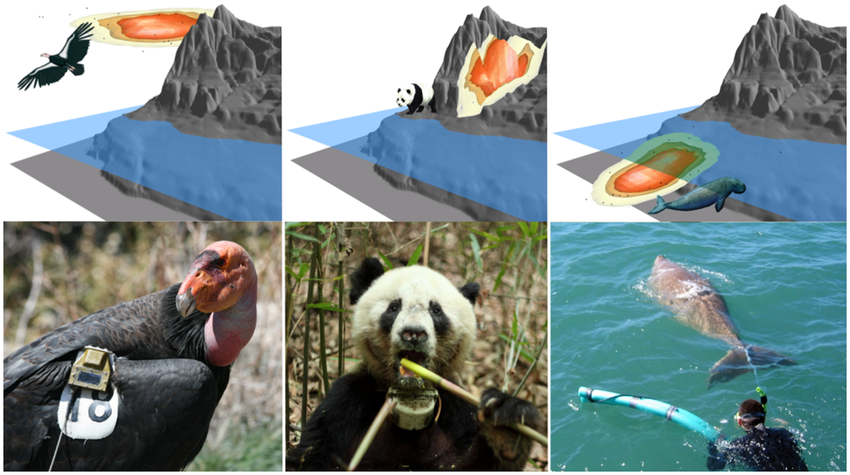
\includegraphics[scale = 0.8]{GPS_animals}
\caption{\scriptsize Examples of avian, terrestrial, and aquatic animal biotelemetry data sets and their spatial domains. Left: California condor with a
GPS biologger attached to its patagium. Center: A giant panda telemetered with a GPS collar. Right: A dugong fitted with a tail mounted GPS biologger. \cite{Tracey2014}}
\end{figure}

 \end{frame}



%============================================
\begin{frame}{Movement ecology}
%============================================



\begin{itemize}
 \item $Y_t$ : characteristic of movement at time $t$. 
 
 \begin{itemize}
 \item Possibly multivariate: speed, depth, angular speed, etc... 
 \end{itemize}
 
 \item \textbf{Idea} : the value of this characteristic depends on the type of activity of the animal at time $t$: travelling, searching for food, sleeping...
 
 \item Let $Z_t$ represent the  behavior state at time $t$: 
 
 $$Y_t | Z_t = k \sim \Fcal(\cdot,\gamma_k)$$
 
 
 \item Time dependeance in $Z_t$ :  Markov  property 

$$P(Z_{t} = z | Z_{t-1} = z_{t-1}, \dots, Z_{1} = z_{1},Z_{0} = z_{0}  )  =
 P(Z_{t} = z | Z_{t-1} = z_{t-1}) $$ 
 
 \end{itemize}






\end{frame}



%============================================
\begin{frame}{Narwhals \cite{Ngo2019} }
%============================================

Understanding narwhal diving behaviour using Hidden Markov Models


\begin{center} 
\begin{minipage}[c]{.46\linewidth}
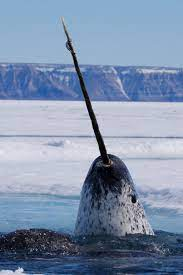
\includegraphics[width= 0.7 \textwidth]{Narwhal}
\end{minipage} \hfill
\begin{minipage}[c]{.46\linewidth}
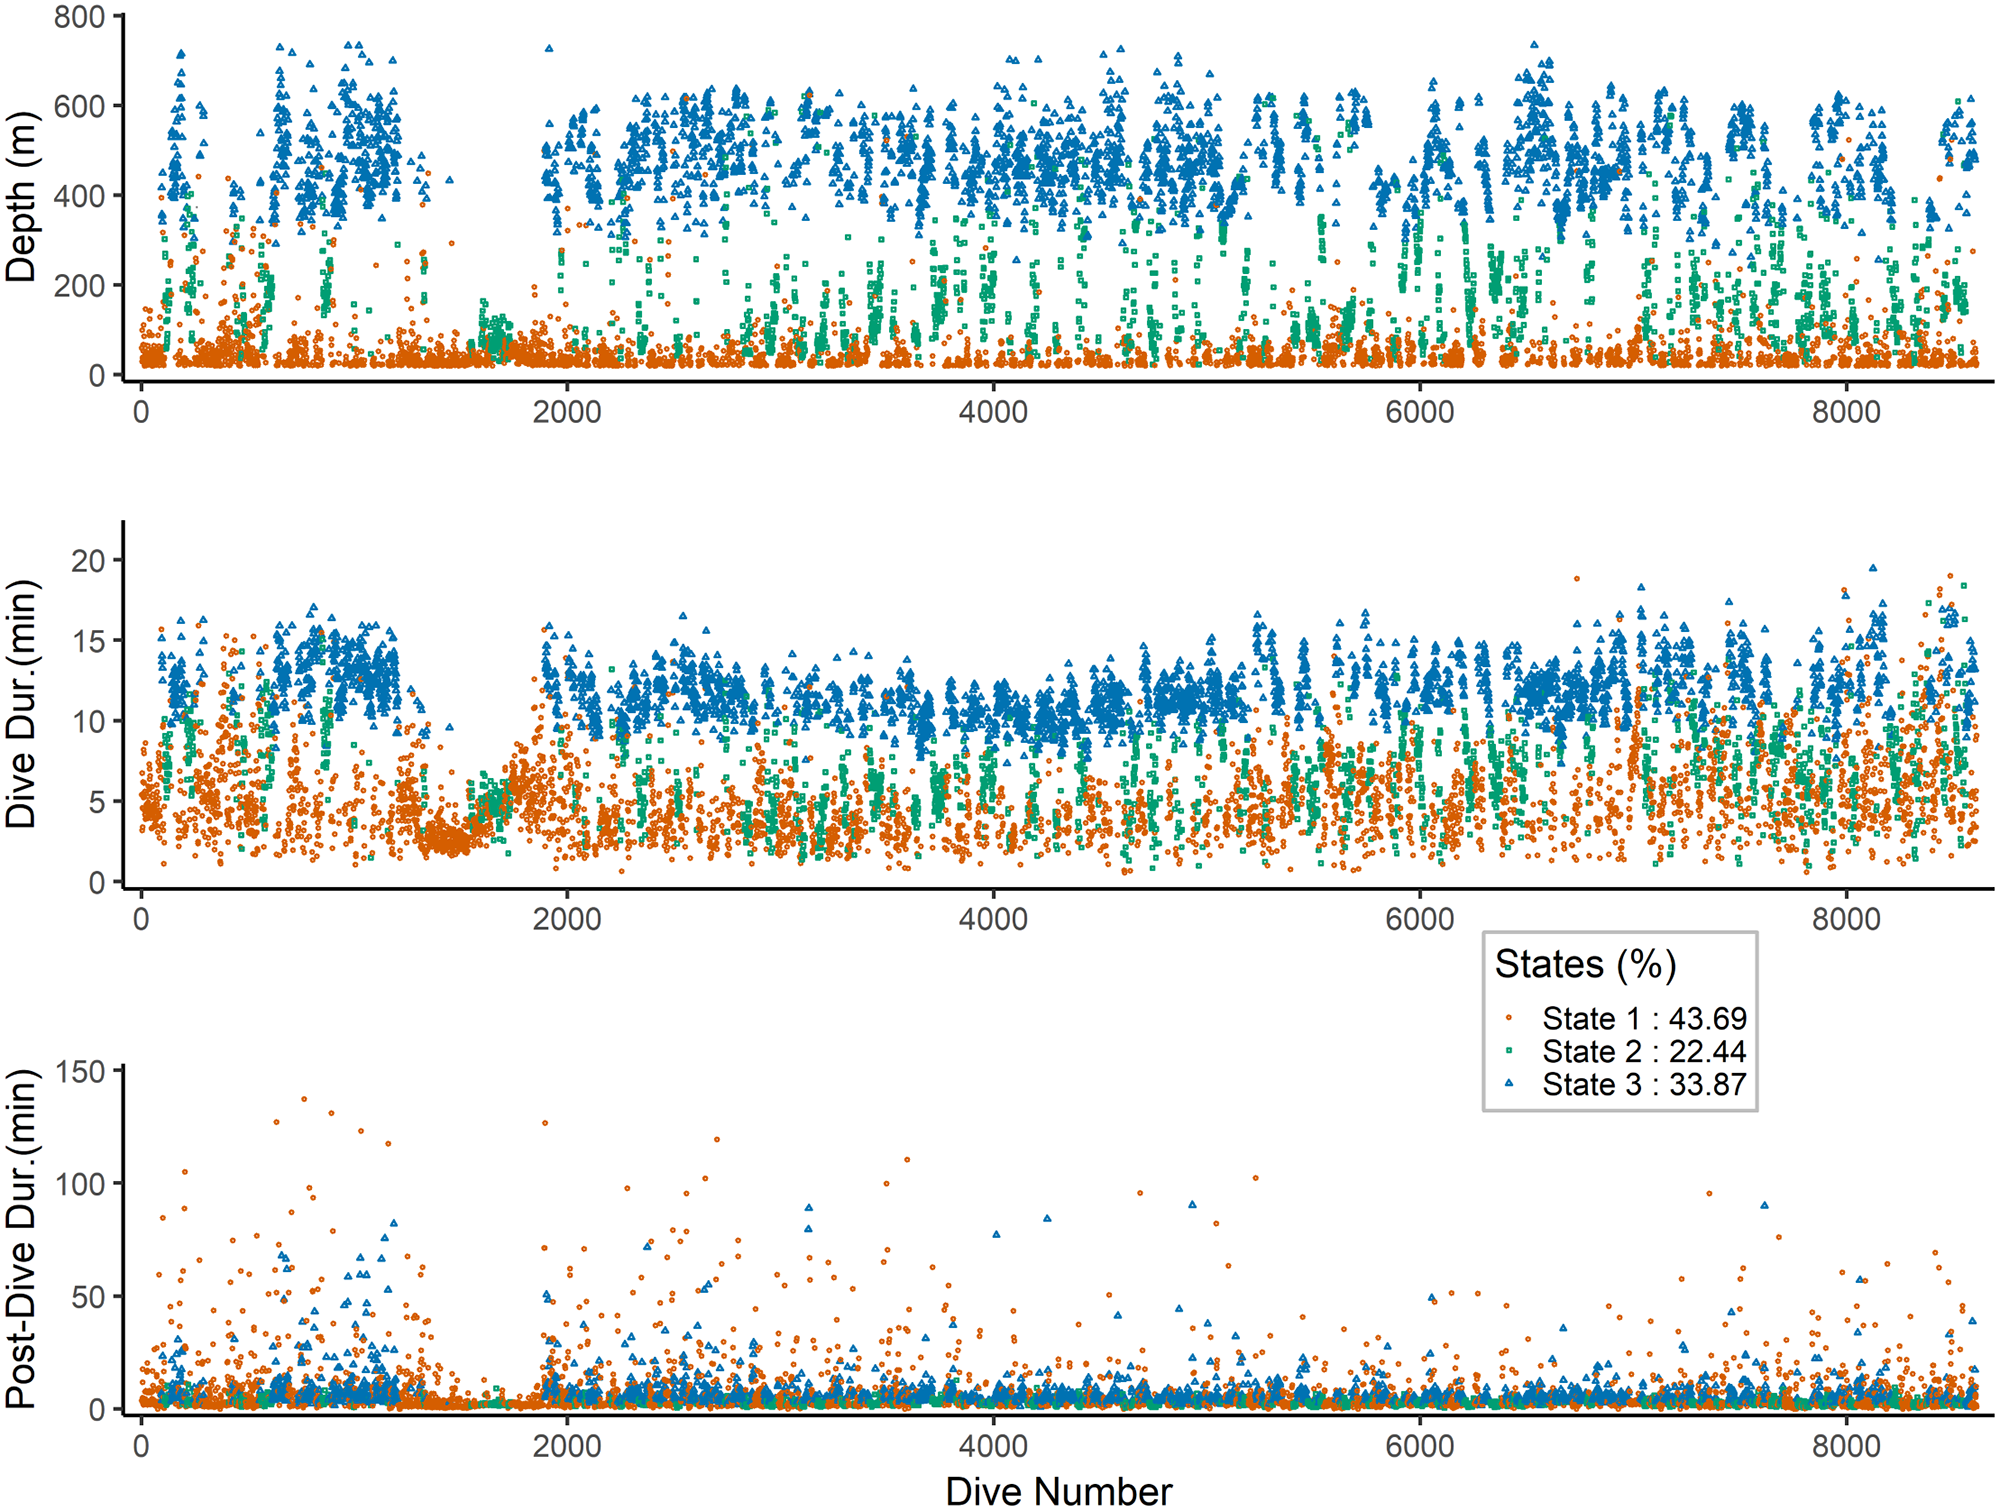
\includegraphics[width=  \textwidth]{InferredNarwhal}
\end{minipage}
\end{center}


\end{frame}



%============================================
\begin{frame}{Albatross \cite{Conners2021}}
%============================================
Hidden Markov models identify major
movement modes in accelerometer and
magnetometer data from four albatros
species
\begin{center} 
\begin{minipage}[c]{.46\linewidth}
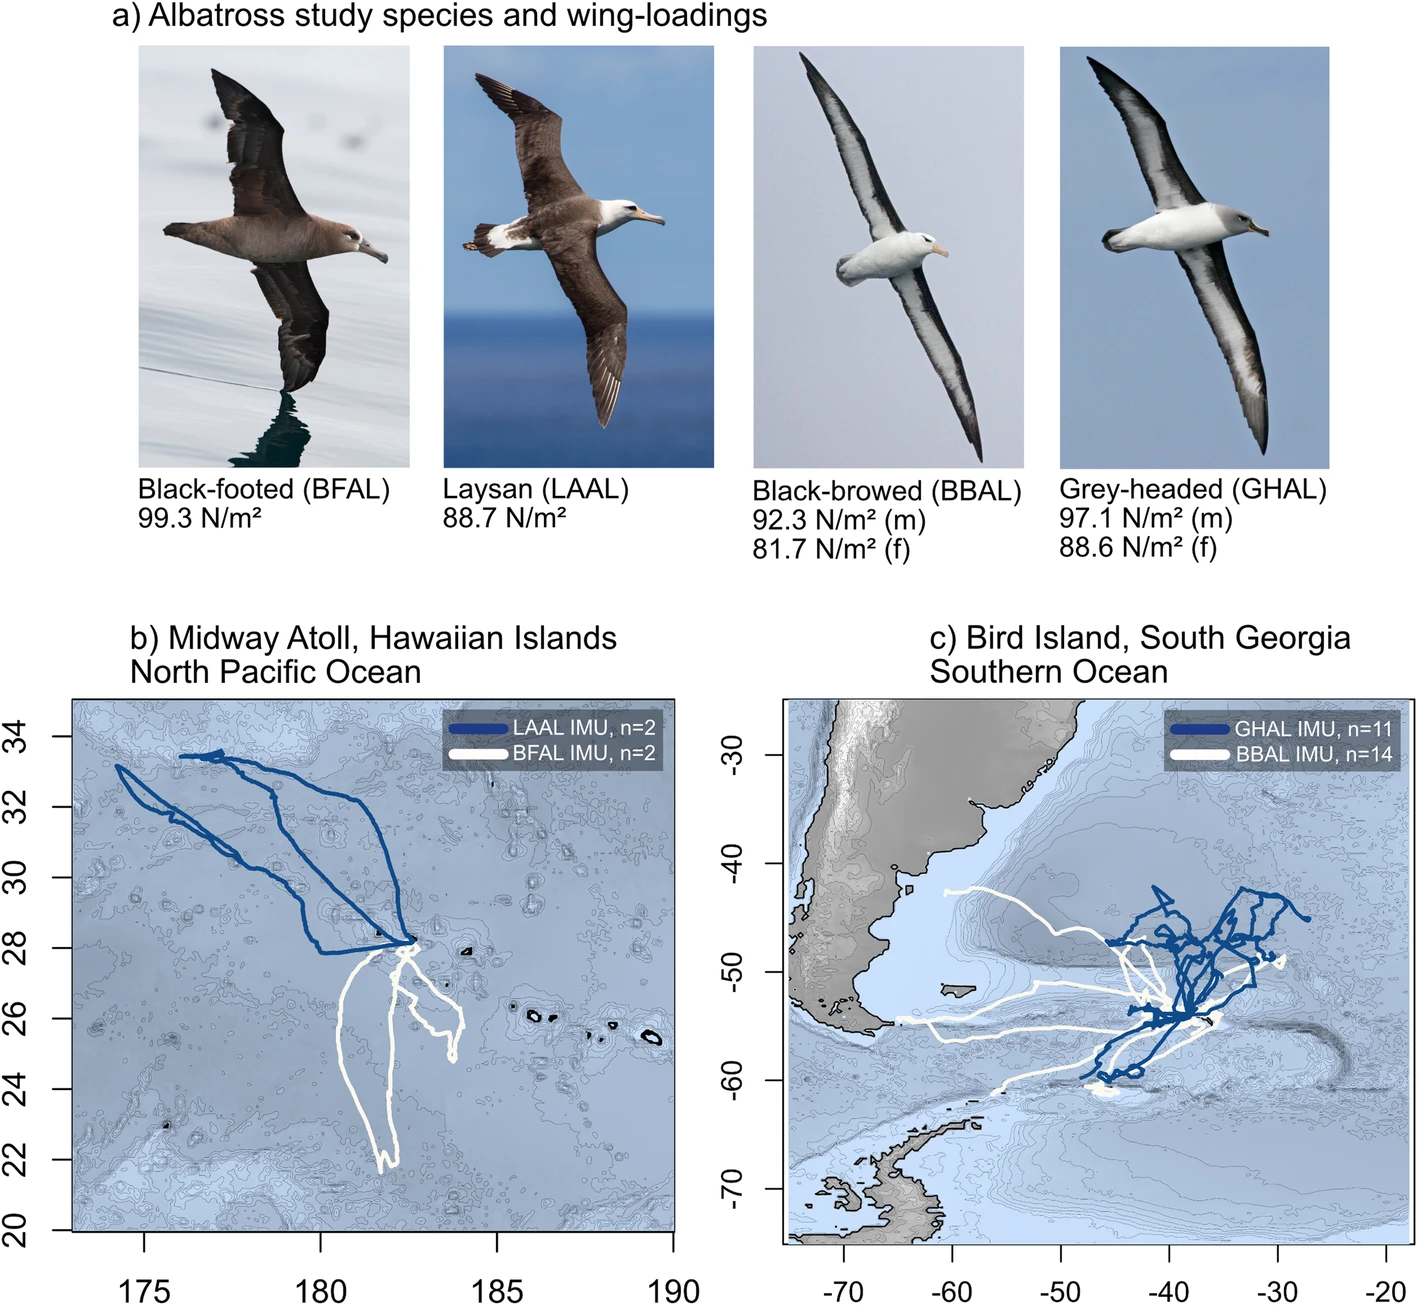
\includegraphics[width= \textwidth]{Albatros1}
\end{minipage} \hfill
\begin{minipage}[c]{.46\linewidth}
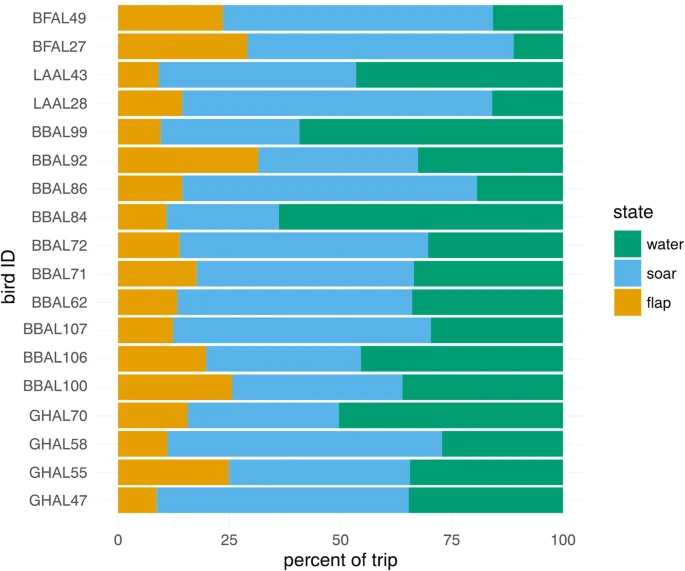
\includegraphics[width=  \textwidth]{Albatros2}
\end{minipage}
\end{center}

 
\end{frame}



%============================================
\begin{frame}{Other animals  \cite{McClintock2018}}
%============================================
\textsf{R}-package for HMM inference. Trajectories of elephants, fur seal... 

\begin{center} 
\begin{minipage}[c]{.46\linewidth}
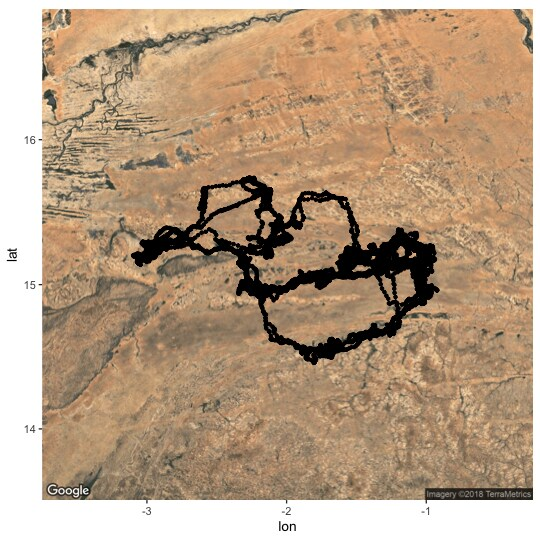
\includegraphics[width= \textwidth]{elephant_plotSat}
\end{minipage} \hfill
\begin{minipage}[c]{.46\linewidth}
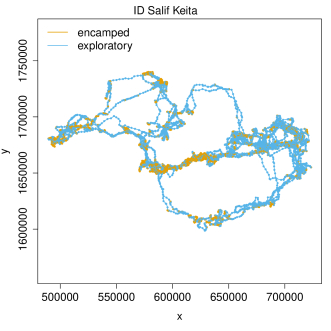
\includegraphics[width=  \textwidth]{inferedElephant}
\end{minipage}
\end{center}
 
 

\end{frame}
%===================================================
\begin{frame}{HMM for Human genetic}
%===================================================

\begin{itemize}
 \item Better understand the genetic structure of populations
 \item Relies on the genotyping of large sets of individuals sampled in different places, environments or with different origins
 \item Genotype $Y_{it}$ of a series of individuals $i \in \interval{1}{I}$ at a series of locus $t \in \interval{1}{T}$ is measured
 \item \textcolor{dgreen}{Aim}: distinguish sub-populations of individuals.
\end{itemize}

\end{frame}


%===================================================
\begin{frame}{HMM model for population genetics}
%===================================================

For each individual $i$ and locus $t$, $Z_{it}$ unknown population origins. 

\begin{itemize}
 \item In Chapter $1$  : $(Z_{it})_t$ are independant
 \item Here, one may assume that the popupulation origins at locus $t$ depends  of the one at locus $t-1$. 
 \item Dependency between neighbor loci
 \end{itemize}

\begin{eqnarray*} 
  (Z_i) & \text{iid} & Z_i = (Z_{i1}, \dots, Z_{iT}), \\
 (Z_{it})_t & \sim & \MC(\nu, \pi), \\
 (Y_{it})_{it} \text{ indep.} \,|\, (Z_{it}) & \sim & F(\gamma_{Z_{it}}),
\end{eqnarray*}
with multinomial emission distribution $F(\gamma_k) = \Mcal(1; \gamma_k)$.
\end{frame}

%
%%===================================================
%\begin{frame}{HMM model for  aligment of biological sequences}
%%===================================================
% 
%See at the end of the chapter 
%\end{frame}


 
\section{Hidden Markov model}

\subsection{Definition of the HMM}
%============================================
\begin{frame}{About Markov Chains}
%============================================
 
$Z_t$ is a Markov Chain on the finite state  space  $\interval{1}{K}$: $
Z_t \sim \MC(\nu, \pi)
$ where 
\begin{itemize}
 \item $\nu = (\nu_1, \dots, \nu_K)$ with  $\nu_k = P(Z_1 = k)$   (initial distribution)
  \item $\pi$ is the $K \times K$ transition matrix:
$$
\pi_{k, \ell} = P(Z_{t+1} = \ell | Z_t = k).
$$
\end{itemize}
\textcolor{dgreen}{A few properties}
\begin{itemize}
 \item Let $\nu_t  = (\nu_{t1}, \dots, \nu_{tK})$  be the distribution of the hidden state at time $t$:
$
\nu_{tk} = P(Z_t = k).
$
Then, $(Z_t)$ being an homogeneous Markov chain, we have
$$
\nu_t = \nu^\intercal \pi^{t-1}
$$

\item If $(Z_t)$ is a \textcolor{dgreen}{stationary Markov chain} i.e. 
$
\nu = \nu^\intercal \pi.
$ 
then $$\nu_t = \nu, \forall t. $$
\end{itemize}
 

 
\end{frame}




%============================================
\begin{frame}{Model}
%============================================
 

\begin{definition} \label{Def:HMM}
  The general hidden Markov chain model is defined as follows:
  \begin{equation} \label{Eq:HMM}
  \begin{array}{rcrcl}
  & & (Z_t)_t & \sim & \MC(\nu, \pi),
  \\
  (Y_t)_t \text{ indep. } | (Z_t), & &
  Y_t | (Z_t = k) & \sim & F_k = F(\gamma_k),
  \end{array}
  \end{equation}
  The Markov chain $\MC(\nu, \pi)$ is defined over the {\sl state space} $\interval{1}{K}$, $K$ being the number of hidden states. 
\end{definition}


\textcolor{dgreen}{Parameters}: $\theta = (\nu, \pi, \gamma)$
\end{frame}



%============================================
\begin{frame}{About the emission distribution}
%============================================
\begin{itemize}
 \item Must be adapted to the data one wants to modelize
 \item If $Y_t \in \R^d$ : multivariate gaussian 
 $$Y_t | Z_t = k \sim \mathcal{M}_d(\mu_k, \Sigma_k)$$
 \item If $Y_t$ is a speed : gamma distribution. 
 \item If $Y_t$ is a speed which can be null : gamma distribution and Dirac mass.
 \item If $Y_t$ is an angular speed : adapted distribution! 
\end{itemize}


 
\end{frame}
 

%============================================
\begin{frame}{Marginal distribution of $Y_t$}
%============================================
$$
Y_t \sim \sum_{k=1}^K \nu_{tk} f(\cdot; \gamma_k).
$$

Indeed: 
 \begin{eqnarray*}
  p(Y_t ) &=& \sum_{k=1}^K p(Y_t | Z_t=k) P(Z_t = k)= \sum_{k=1}^K f(Y_t; \gamma_k) \nu_{tk}
 \end{eqnarray*}

If $(Z_t)$ is stationnary i.e. $\nu_{tk} = \nu_k$ then: 
$
Y_t \sim \sum_{k=1}^K \nu_{k} f(\cdot; \gamma_k).
$





\end{frame}



\subsection{Dependency properties}






%============================================
\begin{frame}{Dependencies structure}
%============================================

We do not have  the same independancy properties as in the mixture model. 

\textcolor{dgreen}{Useful notations:} 
\begin{itemize}
 \item $Z_s^t = (Z_s, \dots Z_t)$ (for $s \leq t$)
 \item $Y_s^t = (Y_s, \dots Y_t)$ 
\end{itemize}


\end{frame}



%============================================
\begin{frame}{DAG of HMM}
 %============================================
\begin{center}
%   \includegraphics[scale=.3, clip=true, trim=0 335 65 0]{../Figures/HMModel}
  \begin{tikzpicture}
  \node[hidden] (Z1) at (0, 0) {$Z_1$};
  \node[empty] (E1) at (.75*\edgeunit, 0) {$\quad$};
  \node[hidden] (Zt) at (1.5*\edgeunit, 0) {$Z_t$};
  \node[hidden] (Zt1) at (2.5*\edgeunit, 0) {$Z_{t+1}$};
  \node[empty] (Et1) at (3.25*\edgeunit, 0) {$\quad$};
  \node[hidden] (Zn) at (4*\edgeunit, 0) {$Z_n$};

  \node[observed] (Y1) at (0, -1*\edgeunit) {$Y_1$};
  \node[observed] (Yt) at (1.5*\edgeunit, -1*\edgeunit) {$Y_t$};
  \node[observed] (Yt1) at (2.5*\edgeunit, -1*\edgeunit) {$Y_{t+1}$};
  \node[observed] (Yn) at (4*\edgeunit, -1*\edgeunit) {$Y_n$};

  \draw[dashedarrow] (Z1) to (E1);
  \draw[dashedarrow] (E1) to (Zt);
  \draw[arrow] (Zt) to (Zt1);
  \draw[dashedarrow] (Zt1) to (Et1);
  \draw[dashedarrow] (Et1) to (Zn);

  \draw[arrow] (Z1) to (Y1);
  \draw[arrow] (Zt) to (Yt);
  \draw[arrow] (Zt1) to (Yt1);
  \draw[arrow] (Zn) to (Yn);

  \end{tikzpicture}
  \end{center}
 
 
\textbf{Factorisation}

$$\mathbb{P}(Y_1, \dots, Y_n, Z_1, \dots, Z_n) = \prod_{t=1}^{n} \mathbb{P}(Y_t | Z_t) \; \mathbb{P}(Z_1) \prod_{t=1}^{n-1} \mathbb{P}(Z_{t+1} | Z_t) $$
\end{frame}

%============================================
\begin{frame}{About directed acyclic graphes (DAG)}
 %============================================
See book by Lauritzen or see \href{https://www.stat.cmu.edu/~larry/=sml/DAGs.pdf}{here}  for an introduction to DAG.

\begin{block}{Factorized distributions}

Let $\mathcal{V} = (V_1, \dots, V_N)$ be  a set of dependant random variables with joint distribution $\mathbb{P}$ and let $\mathcal{G} = (\mathcal{V},E)$ be a directed  acyclic graphe. $\mathbb{P}$  is said to be factorized with respect to $\mathcal{G}$ if 
$$\mathbb{P}(V_1, \dots, V_N) = \prod_{i=1}^N \mathbb{P}(V_i | Pa(V_i,\mathcal{G}))$$
where  $Pa(V_i,\mathcal{G})$ denotes the parents of node $V_i$ in $\mathcal{G}$. 
\end{block}
\end{frame}



%============================================
\begin{frame}{Other example}
 %============================================
\begin{center}
%   \includegraphics[scale=.3, clip=true, trim=0 335 65 0]{../Figures/HMModel}
  \begin{tikzpicture}
  \node[observed] (X5) at (0, 0) {$X_5$};
  \node[observed] (X2) at (1.5*\edgeunit, 0) {$X_2$};
  \node[observed] (X3) at (3*\edgeunit, 0) {$X_{3}$};
  \node[observed] (X4) at (4*\edgeunit, 1*\edgeunit) {$X_4$};
  \node[observed] (X1) at (1.5*\edgeunit, -1*\edgeunit) {$X_1$};
  

  \draw[arrow] (X5) to (X1);
  \draw[arrow] (X2) to (X1);
  \draw[arrow] (X3) to (X1);
  \draw[arrow] (X4) to (X3);
   

  \end{tikzpicture}
  \end{center}
 
 
$$\mathbb{P}(X_1,X_2,X_3,X_4,X_5) = \mathbb{P}(X_1 |X_2,X_3,X_5)\mathbb{P}(X_2)\mathbb{P}(X_5)\mathbb{P}(X_3|X_4)\mathbb{P}(X_4)$$
\end{frame}

%============================================
\begin{frame}{Moralization of a DAG}
%============================================
\begin{block}{Moral graphe}
The moral version of a graphe $\mathcal{G}$ is obtained by marrying the parents and by removing the directions on the edges. 
\end{block}



% 
% \begin{center}
% %   \includegraphics[scale=.3, clip=true, trim=0 335 65 0]{../Figures/HMModel}
%   \begin{tikzpicture}
%   \node[observed] (X5) at (0, 0) {$X_5$};
%   \node[observed] (X2) at (1.5*\edgeunit, 0) {$X_2$};
%   \node[observed] (X3) at (3*\edgeunit, 0) {$X_{3}$};
%   \node[observed] (X4) at (4*\edgeunit, 1*\edgeunit) {$X_4$};
%   \node[observed] (X1) at (1.5*\edgeunit, -1*\edgeunit) {$X_1$};
%   \draw[arrow] (X5) to (X1);
%   \draw[arrow] (X2) to (X1);
%   \draw[arrow] (X3) to (X1);
%   \draw[arrow] (X4) to (X3);
%   \end{tikzpicture}
% \end{center}
%   
  
  \begin{center}
%   \includegraphics[scale=.3, clip=true, trim=0 335 65 0]{../Figures/HMModel}
  \begin{tikzpicture}
  \node[observed] (X5) at (0, 0) {$X_5$};
  \node[observed] (X2) at (1.5*\edgeunit, 0) {$X_2$};
  \node[observed] (X3) at (3*\edgeunit, 0) {$X_{3}$};
  \node[observed] (X4) at (4*\edgeunit, 1*\edgeunit) {$X_4$};
  \node[observed] (X1) at (1.5*\edgeunit, -1*\edgeunit) {$X_1$};
  
  \draw[line width=1.5pt]   (X5) -- (X2);
  \draw[line width=1.5pt]  (X3) -- (X2);
  \draw[line width=1.5pt]     (X5) to[bend left] (X3);
  
  \draw[line width=1.5pt]  (X1) -- (X5);
  \draw[line width=1.5pt]  (X2) -- (X1);
  \draw[line width=1.5pt]  (X3) -- (X1);
  \draw[line width=1.5pt]  (X4) -- (X3);
   

  \end{tikzpicture}
  \end{center}
  
 \end{frame}
 
 
%============================================
\begin{frame}{Moralization of a DAG}
%============================================
\begin{block}{Independancy properties}
Let $I$, $J$ and $K$, 3 subsets of $\mathcal{V}$. 

\begin{enumerate}
 \item In the moral graph deduced from $\mathcal{G}$, if all the paths from $I$ to $J$ pass through  $K$ then 
 $$ (X_i)_{i \in I} \indep  (X_j)_{j \in J} | (X_k)_{k \in K}.$$
\item In a DAG, conditionnally to its parents, a variable is independant from its non-descendant. 
\end{enumerate}


\vspace{1em}  
 
\end{block}

\textbf{Consequence of 1.}
\begin{eqnarray*}
 P(X_I | X_J, X_K) &=& \frac{P(X_I , X_J |  X_K)}{P(X_J | X_K)} =  \frac{P(X_I  | X_K)P(X_J | X_K)}{P(X_J | X_K)} = P(X_I  | X_K) 
\end{eqnarray*}

\end{frame}

 
%============================================
\begin{frame}{Example}
%============================================

\begin{enumerate}
 \item $I = \{5,2,1\}, J = \{4\}, K = \{3\}$
 $$P(X_5,X_2,X_1,X_4 | X_3) = P(X_5,X_2,X_1 | X_3) P(X_4 | X_3)$$
 \item $P(X_1 | X_2,X_3,X_4,X_5) = P(X_1 | X_2,X_3,X_5) $
 \end{enumerate}
\end{frame}

 
%============================================
\begin{frame}{Application for HMM}
\begin{center}
%   \includegraphics[scale=.3, clip=true, trim=0 335 65 0]{../Figures/HMModel}
  \begin{tikzpicture}
  \node[hidden] (Z1) at (0, 0) {$Z_1$};
  \node[empty] (E1) at (.75*\edgeunit, 0) {$\quad$};
  \node[hidden] (Zt) at (1.5*\edgeunit, 0) {$Z_t$};
  \node[hidden] (Zt1) at (2.5*\edgeunit, 0) {$Z_{t+1}$};
  \node[empty] (Et1) at (3.25*\edgeunit, 0) {$\quad$};
  \node[hidden] (Zn) at (4*\edgeunit, 0) {$Z_n$};

  \node[observed] (Y1) at (0, -1*\edgeunit) {$Y_1$};
  \node[observed] (Yt) at (1.5*\edgeunit, -1*\edgeunit) {$Y_t$};
  \node[observed] (Yt1) at (2.5*\edgeunit, -1*\edgeunit) {$Y_{t+1}$};
  \node[observed] (Yn) at (4*\edgeunit, -1*\edgeunit) {$Y_n$};

  \draw[dashed width=1pt] (Z1) -- (E1);
  \draw[dashed width=1pt] (E1) -- (Zt);
  \draw[line width=1pt] (Zt) -- (Zt1);
  \draw[line width=1pt] (Zt1) -- (Et1);
  \draw[dashed width=1pt] (Et1) -- (Zn);

  \draw[line width=1pt] (Z1) -- (Y1);
  \draw[line width=1pt] (Zt) -- (Yt);
  \draw[line width=1pt] (Zt1) -- (Yt1);
  \draw[line width=1pt] (Zn) -- (Yn);

  \end{tikzpicture}
  \end{center}
 

 
\begin{enumerate}

 \item $p(Z_{t+1} | Y_1^t, Z_1^t) = p(Z_{t+1} |Z_t)$
 \item $p(Z_{t+1} |  Z_1^t)  = p( Z_{t+1} |Z_t)$
 $$I = \{Y_{t+1}\}, K = \{Z_{t+1}\}, J = \{Z_{1}^{t-1},, Y_{1}^t\}$$
 \item $p(Y_{t+1} | Y_1^t, Z_1^{t+1}) = p(Y_{t+1} | Z_{t+1})$ 
\end{enumerate}

\end{frame}

%============================================
 
 
 
\begin{frame}{Application for HMM}

\textcolor{dgreen}{Consequences} 
\begin{enumerate}[($a$)]
 \item all paths from $Y_1^t$ to $Z_{t+1}$ go through $Z_1^t$  \textcolor{dgreen}{$\Rightarrow$}  
 $Z_{t+1} $ is independent from $Y_1^t$ conditionally on $Z_1^t$
 $$p(Z_{t+1} | Y_1^t, Z_t) = p(Z_{t+1} |Z_t)$$
\item all paths from $Z_1^{t-1}$ to $Z_{t+1}$ go through $Z_t$, meaning that $Z_{t+1}$ is independent from $Z_1^{t-1}$ conditionally on $Z_t$ (i.e. $(Z_t)$ is a Markov chain);
 \item all paths from $Y_1^t$ to $Y^{t+1}$ go through $Z_ {t+1}$ meaning that $Y^{t+1}$ is independent from $Y_1^t$ to  conditionally on $Z_ {t+1}$ %(and the same holds with $Z_t$).
 $$p(Y_{t+1} | Y_1^t, Z_{t+1}) = p(Y_{t+1} |Z_{t+1})$$
 %$$p(Z_{t+1} | Y_1^t, Y_{t+1}) = p(Z_{t+1} |Y_{t+1})$$
\end{enumerate}

\end{frame}

%============================================
\begin{frame}{Property}
%============================================
 
  
\begin{proposition}
 $(Z_t)$ conditional on the observed data $\bY = Y_1^n$
is still a Markov chain. \underline{And}  
$$p(Z_{t+1} | Z_{1}^t, Y_{1}^n) = p(Z_{t+1} | Z_t, Y_{t+1}^n)$$

\end{proposition}
\end{frame}
%============================================
\begin{frame}{Proof (i)}
%============================================

\begin{center}
%   \includegraphics[scale=.3, clip=true, trim=0 335 65 0]{../Figures/HMModel}
  \begin{tikzpicture}
  \node[hidden] (Z1) at (0, 0) {$Z_1$};
  \node[empty] (E1) at (.75*\edgeunit, 0) {$\quad$};
  \node[hidden] (Zt) at (1.5*\edgeunit, 0) {$Z_t$};
  \node[hidden] (Zt1) at (2.5*\edgeunit, 0) {$Z_{t+1}$};
  \node[empty] (Et1) at (3.25*\edgeunit, 0) {$\quad$};
  \node[hidden] (Zn) at (4*\edgeunit, 0) {$Z_n$};

  \node[observed] (Y1) at (0, -1*\edgeunit) {$Y_1$};
  \node[observed] (Yt) at (1.5*\edgeunit, -1*\edgeunit) {$Y_t$};
  \node[observed] (Yt1) at (2.5*\edgeunit, -1*\edgeunit) {$Y_{t+1}$};
  \node[observed] (Yn) at (4*\edgeunit, -1*\edgeunit) {$Y_n$};

  \draw[dashed, line width=1pt] (Z1) -- (E1);
  \draw[dashed, line width=1pt] (E1) -- (Zt);
  \draw[line width=1pt] (Zt) -- (Zt1);
  \draw[dashed, line width=1pt] (Zt1) -- (Et1);
  \draw[dashed, line width=1pt] (Et1) -- (Zn);

  \draw[line width=1pt] (Z1) -- (Y1);
  \draw[line width=1pt] (Zt) -- (Yt);
  \draw[line width=1pt] (Zt1) -- (Yt1);
  \draw[line width=1pt] (Zn) -- (Yn);

  \end{tikzpicture}
  \end{center}
 
  
\textbf{Use DAG properties (Exercice)} or :   
\begin{eqnarray*}
p(Z_{t+1} | Z_1^t, Y_1^n) 1&=& p(Z_{t+1} | Z_1^t, Y_{1}^t, Y_{t+1}^n) =  \frac{p(Z_{t+1} ,  Z_1^t, Y_{1}^t, Y_{t+1}^n)}{p( Z_1^t, Y_{1}^t, Y_{t+1}^n)} \\
 &=& \frac{p(Y_{t+1}^n |\cancel{Y_{1}^t}, Z_{t+1} ,  \cancel{Z_1^t} )p(Y_{1}^t , Z_{t+1} ,  Z_1^t )}{p( Y_{t+1}^n| Z_1^t, Y_{1}^t)p(Z_1^t, Y_{1}^t)} 
\\
& = & \frac{p(Y_{t+1}^n | Z_{t+1} )p(Y_{1}^t | Z_{t+1} ,  Z_1^t )p(Z_{t+1} | Z_{\Ccancel[blue]{1}}^t )\Ccancel[orange]{p(Z_1^t)}}
{p( Y_{t+1}^n| Z_1^t, Y_{1}^t)p(Y_{1}^t|Z_1^t)\Ccancel[orange]{p(Z_1^t )}}   
\end{eqnarray*}

\end{frame}
%============================================
\begin{frame}{Proof (ii)}
%============================================

 \begin{center}
%   \includegraphics[scale=.3, clip=true, trim=0 335 65 0]{../Figures/HMModel}
  \begin{tikzpicture}
  \node[hidden] (Z1) at (0, 0) {$Z_1$};
  \node[empty] (E1) at (.75*\edgeunit, 0) {$\quad$};
  \node[hidden] (Zt) at (1.5*\edgeunit, 0) {$Z_t$};
  \node[hidden] (Zt1) at (2.5*\edgeunit, 0) {$Z_{t+1}$};
  \node[empty] (Et1) at (3.25*\edgeunit, 0) {$\quad$};
  \node[hidden] (Zn) at (4*\edgeunit, 0) {$Z_n$};

  \node[observed] (Y1) at (0, -1*\edgeunit) {$Y_1$};
  \node[observed] (Yt) at (1.5*\edgeunit, -1*\edgeunit) {$Y_t$};
  \node[observed] (Yt1) at (2.5*\edgeunit, -1*\edgeunit) {$Y_{t+1}$};
  \node[observed] (Yn) at (4*\edgeunit, -1*\edgeunit) {$Y_n$};

  \draw[dashed, line width=1pt] (Z1) -- (E1);
  \draw[dashed, line width=1pt] (E1) -- (Zt);
  \draw[line width=1pt] (Zt) -- (Zt1);
  \draw[dashed, line width=1pt] (Zt1) -- (Et1);
  \draw[dashed, line width=1pt] (Et1) -- (Zn);

  \draw[line width=1pt] (Z1) -- (Y1);
  \draw[line width=1pt] (Zt) -- (Yt);
  \draw[line width=1pt] (Zt1) -- (Yt1);
  \draw[line width=1pt] (Zn) -- (Yn);

  \end{tikzpicture}
  \end{center}
 
  
But $p(Y_{1}^t | Z_{t+1} ,  Z_1^t )= p(Y_{1}^t |Z_1^t )$
So
\begin{eqnarray*}
p(Z_{t+1} | Z_1^t, Y_1^n)&=& \frac{p(Y_{t+1}^n | Z_{t+1} )\Ccancel[red]{p(Y_{1}^t | \Ccancel{Z_{t+1}} ,  Z_1^t )}p(Z_{t+1} | Z_{t} )}
{p( Y_{t+1}^n| Z_1^t, Y_{1}^t)\Ccancel[red]{p(Y_{1}^t|Z_1^t)}}   
\end{eqnarray*}
\end{frame}
%============================================
\begin{frame}{Proof (iii)}
%============================================

 \begin{center}
%   \includegraphics[scale=.3, clip=true, trim=0 335 65 0]{../Figures/HMModel}
  \begin{tikzpicture}
  \node[hidden] (Z1) at (0, 0) {$Z_1$};
  \node[empty] (E1) at (.75*\edgeunit, 0) {$\quad$};
  \node[hidden] (Zt) at (1.5*\edgeunit, 0) {$Z_t$};
  \node[hidden] (Zt1) at (2.5*\edgeunit, 0) {$Z_{t+1}$};
  \node[empty] (Et1) at (3.25*\edgeunit, 0) {$\quad$};
  \node[hidden] (Zn) at (4*\edgeunit, 0) {$Z_n$};

  \node[observed] (Y1) at (0, -1*\edgeunit) {$Y_1$};
  \node[observed] (Yt) at (1.5*\edgeunit, -1*\edgeunit) {$Y_t$};
  \node[observed] (Yt1) at (2.5*\edgeunit, -1*\edgeunit) {$Y_{t+1}$};
  \node[observed] (Yn) at (4*\edgeunit, -1*\edgeunit) {$Y_n$};

  \draw[dashedarrow] (Z1) to (E1);
  \draw[dashedarrow] (E1) to (Zt);
  \draw[arrow] (Zt) to (Zt1);
  \draw[dashedarrow] (Zt1) to (Et1);
  \draw[dashedarrow] (Et1) to (Zn);

  \draw[arrow] (Z1) to (Y1);
  \draw[arrow] (Zt) to (Yt);
  \draw[arrow] (Zt1) to (Yt1);
  \draw[arrow] (Zn) to (Yn);

  \end{tikzpicture}
  \end{center}
Moreover
\begin{eqnarray*}
p(Y_{t+1}^n| Z_1^t, Y_{1}^t)&=&\sum_{k=1}^K p( Y_{t+1}^n| \cancel{Z_1^t, Y_{1}^t},Z_{t+1}=k)p(Z_{t+1}=k | Z_{\cancel{1}}^t, \cancel{Y_{1}^t})\\
&=& p(Y_{t+1}^n| Z_t)
\end{eqnarray*}
\end{frame}
%============================================
\begin{frame}{Proof (iv)}
%============================================


Finally: 
\begin{eqnarray*}
p(Z_{t+1} | Z_1^t, Y_1^n) &=& \frac{p(Y_{t+1}^n | Z_{t+1} )\Ccancel[red]{p(Y_{1}^t | \Ccancel{Z_{t+1}} ,  Z_1^t )}p(Z_{t+1} | Z_{t} )}{p( Y_{t+1}^n| Z_1^t, Y_{1}^t)\Ccancel[red]{p(Y_{1}^t|Z_1^t)}}\\
&=& \frac{p(Y_{t+1}^n | Z_{t+1})p(Z_{t+1} | Z_{t} )}{p(Y_{t+1}^n| Z_t)} \\
&=& p(Z_{t+1} | Z_t, Y_{t+1}^n)
\end{eqnarray*}
\end{frame}

\section{Parameters estimation}
%============================================
\begin{frame}{Complete log-likelihood}
%============================================
\textcolor{dgreen}{Notations}:   $\bY = Y_1^n, \quad   \bZ = Z_{1}^n$
\begin{eqnarray*}
\log p_\theta(\bY, \bZ) & = & \log \left[p_\theta(\bZ) p_\theta(\bY|\bZ)\right] \\
&=& \log  p_\theta(Z_1) p_\theta(Y_1|Z_1) + \sum_{t=2}^n \left[ \log  p_\theta(Z_t | Z_{t-1}) + \log  p_\theta(Y_t|Z_t)\right]\\
%  & = & \log \left[\left(\prod_k \nu_k^{Z_{1k}} \prod_{t \geq 2} \prod_{k, \ell} \pi_{k\ell}^{Z_{t-1, k} Z_{t, \ell}}\right)  \left(\prod_{t, k} f(Y_t; \gamma_k)^{Z_{tk}}\right)\right] \\
  & = & \sum_{k=1}^K Z_{1k} \log \nu_k + \sum_{t =2}^n \sum_{k, \ell=1 }^K {Z_{t-1, k} Z_{t, \ell}} \log \pi_{k\ell}\\
&&  + \sum_{t=1, k=1}^{n,K} {Z_{tk} \log f(Y_t; \gamma_k)}.
\end{eqnarray*}

\label{HMM:completell}

\end{frame}
%============================================
\begin{frame}{Marginal (or 'observed') log-likelihood}
%============================================
 
\begin{eqnarray*}
\log p_\theta(\bY) & = & \log \left[\sum_\bZ p_\theta(\bZ) p_\theta(\bY|\bZ)\right] \\
 & = & \log \left[\sum_Z \left(\prod_k \nu_k^{Z_{1k}} \prod_{t \geq 2} \prod_{k, \ell} \pi_{k\ell}^{Z_{t-1, k} Z_{t, \ell}}\right)  \left(\prod_{t, k} f(Y_t; \gamma_k)^{Z_{tk}}\right)\right].
\end{eqnarray*}
\end{frame}

 
%============================================
\begin{frame}{EM algorithm : reminder}
%============================================

$$
\widehat{\theta} = \arg\max_\theta \log p_\theta(\bY).
$$
\label{Algo:EM}

\begin{algorithm}[EM] 
 Repeat until convergence:
  \begin{itemize}
   \item \textcolor{dgreen}{Expectation step:} given the current estimate $\theta^h$ of $\theta$, compute $p_{\theta^h}(\bZ|\bY)$, or at least all the quantities needed to compute $\Esp_{\theta^h}\left[\log p_\theta(\bY, \bZ) |\bY\right]$;
   \item \textcolor{dgreen}{Maximization step:} update the estimate of $\theta$ as
   $$
   \theta^{h+1} = \arg\max_\theta \Esp_{\theta^h}[\log p_\theta(\bY, \bZ) |\bY].
   $$
  \end{itemize}
\end{algorithm}
\end{frame}

%============================================
\begin{frame}{E-step: compute $\Esp_{\theta^{(h)}}[\log p_\theta(Y, Z) | Y]$}
%============================================
Using Slide \ref{HMM:completell}
\begin{eqnarray*}
&&\Esp[\log p_\theta(\bY, \bZ) | \bY]   =\Esp\left[ \sum_{k=1}^K Z_{1k} \log \nu_k + \sum_{t =2}^n \sum_{k, \ell=1 }^K {Z_{t-1, k} Z_{t, \ell}} \log \pi_{k\ell}|\bY \right]\\
&&  + \Esp\left[\sum_{t=1, k=1}^{n,K} {Z_{tk} \log f(Y_t; \gamma_k)}|\bY \right].\\
&=&   \sum_{k=1}^K \tau_{1k} \log \nu_k + \sum_{t=2}^n \sum_{k, \ell=1}^K \eta_{tk\ell} \log \pi_{k\ell} + \sum_{t=1, k=1}^{n,K} {\tau_{tk} \log f(Y_t; \gamma_k)}
\end{eqnarray*}
where
\begin{eqnarray*}
\tau_{tk}& =& \Esp[Z_{tk} | \bY] = P(Z_t = k|\bY)\\
\eta_{tk\ell} &=& \Esp[Z_{t-1, k} Z_{t, \ell} | \bY] = P(Z_{t-1} = k, Z_t = \ell | \bY).
\end{eqnarray*}
\end{frame}
 
%============================================
\begin{frame}{Remark}
%============================================
As opposed to the mixture model:  
$$\tau_{tk} = P(Z_t = k | \bY) \neq P(Z_t = k | Y_t)$$


More generally, $p(\bZ|\bY)$ does not factorize over $t$ any more.
\end{frame}


%============================================
\begin{frame}{Foward- backward formulae}
%============================================
\begin{proposition} \label{Prop:ForBack}
 The conditional probabilities $\tau_{tk}$ and $\eta_{tk\ell}$ can be computed via the two following recursions.
 \begin{itemize}
  \item \textcolor{dgreen}{Forward   (for $t=1, \dots, n$):} Denoting $F_{tk} = P_\theta(Z_t=k | Y_1^t)$ compute
  \begin{eqnarray*}
    F_{1\ell} & \propto & \nu_\ell f_\ell(Y_1)\\
    F_{t\ell}  &\propto&  f_\ell(Y_t) \sum_{k=1}^K F_{t-1, k} \pi_{k\ell} 
  \end{eqnarray*}
  such that, for all $t: \sum_{k =1}^KF_{t\ell} = 1$.
  \item\textcolor{dgreen}{Backward   (for $t=n, \dots, 1$)} 
\begin{eqnarray*}
\tau_{nk} &=& P(Z_n=k | \bY) = P_\theta(Z_n=k | Y_1^n) = F_{nk}\\
  G_{t+1, \ell} &=& \sum_{k=1}^K \pi_{k \ell} F_{tk}, \qquad
  \eta_{tk\ell} = \pi_{k \ell} \frac{\tau_{t+1, \ell}}{G_{t+1, \ell}}
  F_{tk}, \qquad \tau_{tk} = \sum_{\ell=1}^K \eta_{tk\ell}.
  \end{eqnarray*}
 \end{itemize}
\end{proposition}


\end{frame}


%============================================
\begin{frame}[allowframebreaks]{Proof of the Forward formula}
%============================================
For $t=1$ 
  \begin{eqnarray*} 
  {F_{1\ell}} &=& P(Z_{1} = \ell|Y_1) \\
&=& p(Y_1|Z_1 = \ell) P(Z_1 = \ell) \left/p(Y_1) \right.\\
&\propto& \nu_\ell f_\ell(Y_1)   \quad (F1)
\end{eqnarray*}
by the Bayes Formula. 

For $t \geq 2$
  \begin{eqnarray*} 
    {F_{t\ell}} & = & P(Z_t =\ell| Y_1^t) \quad 
    \; = \; \sum_{k=1}^K P(Z_{t-1} = k, Z_t = \ell | Y_1^t) \\
    & = & \sum_{k=1}^K \frac{p(Z_t = \ell, Z_{t-1} = k, Y_1^t)}{p(Y_1^t)} \\ 
    & = &\sum_{k=1}^K \frac{
\overbrace{p(Y_1^{t-1})}^{\indep k} \overbrace{P(Z_{t-1} = k |Y_1^{t-1})}^{ {F_{t-1 k}} }  \overbrace{P(Z_ t =  \ell|Z_{t-1} = k)}^{\pi_{k,\ell}} \overbrace{p(Y_t | Z_t = \ell)}^{\indep k \mbox{ and }  = f_\ell(Y_t)} }{p(Y_1^t)}  \\
    & & \text{(using conditional independences, from the past to present $t$)} \\
    & = & \frac{p(Y_1^{t-1})}{p(Y_1^t)} {f_{\ell}(Y_t)  \sum_{k=1}^K \pi_{k \ell} F_{t-1, k}} \\
 F_{t\ell} &= & P(Z_t =\ell| Y_1^t)  \propto f_{\ell}(Y_t)  \sum_{k=1}^K \pi_{k \ell} F_{t-1, k}   \quad (F2)
  \end{eqnarray*}
\end{frame}



%============================================
\begin{frame}[allowframebreaks]{About the normalizing constant}
%============================================

Note that  $$\sum_{\ell=1}^K F_{t\ell} = \sum_{\ell=1}^K P(Z_t =\ell| Y_1^t)=1$$
So 
\begin{eqnarray*}
 &&\sum_{\ell=1}^K \frac{p(Y_1^{t-1})}{p(Y_1^t)} {f_{\ell}(Y_t)  \sum_{k=1}^K \pi_{k \ell} F_{t-1, k}} =1 \\
 &\Leftrightarrow& \frac{p(Y_1^{t-1})}{p(Y_1^t)}\sum_{\ell=1}^K{f_{\ell}(Y_t)  \sum_{k=1}^K \pi_{k \ell} F_{t-1, k}} =1\\
 &\Leftrightarrow&\frac{p(Y_1^{t})}{p(Y_1^{t-1})} =   \sum_{\ell=1}^K{f_{\ell}(Y_t)  \sum_{k=1}^K \pi_{k \ell} F_{t-1, k}}
 \end{eqnarray*}

$$ 
\frac{p(Y_1^{t})}{p(Y_1^{t-1})}  = \frac{p(Y_1^{t-1},Y_t)}{p(Y_1^{t-1})} = p(Y_t | Y_1^{t-1})$$
 
\begin{block}{Useful formula}
 \begin{equation}\label{HMM:eq lik}
p(Y_t | Y_1^{t-1}) =   \sum_{\ell=1}^K{f_{\ell}(Y_t)  \sum_{k=1}^K \pi_{k \ell} F_{t-1, k}}                                                         \end{equation}
\end{block}

\hyperlink{HMM: eq:marg like}{\beamergotobutton{Use of the formula to compute the marginal likelihood}}

\end{frame}



%============================================
\begin{frame}[allowframebreaks]{Proof of the Backward formula}
%============================================
 The initialization is given by the last step of the forward recursion:
  $$
  {\tau_{nk}} = P(Z_n =k|\bY) = P(Z_n =k|Y_1^n) = {F_{nk}}
  $$
  and the recursion follows as: for $t \leq n-1$
  \begin{eqnarray*} 
    {\tau_{tk}} & = & P(Z_t = k| Y_1^n) = \sum_{\ell=1}^K \underset{\eta_{tk\ell}}{\underbrace{P(Z_t = k, Z_{t+1} = \ell | Y_1^n)}}  = \sum_{\ell=1}^K \eta_{tk\ell} \quad (B3) \\
   \eta_{tk\ell} & = &  \frac{\overbrace{P(Z_t = k, Z_{t+1} = \ell, Y_1^n)}^{\textcolor{dgreen}{(\bullet)}} }{p(Y_1^n)}
\end{eqnarray*}
with 
 \begin{eqnarray*} 
\textcolor{dgreen}{(\bullet)} &=&P(Z_t = k, Z_{t+1} = \ell, Y_1^n)=  P(Z_t = k, Z_{t+1} = \ell, Y_1^t, Y_{t+1}^n) \\
&=&  p(Y_{t+1}^n|Z_{t+1} = \ell, \cancel{Z_{t} = k},  \cancel{Y_{1}^n}) \overbrace{p(Z_{t+1} = \ell| Z_{t} = k,  \cancel{Y_{1}^t})}^{\pi_{k\ell}}\\
&& \underbrace{P(Z_{t} = k |  Y_{1}^t)}_{=F_{tk}}  p(Y_{1}^t)
 \end{eqnarray*}

And so: 

 \begin{eqnarray*} 
 \eta_{tk\ell}  &=& \frac{\textcolor{dgreen}{(\bullet)}}{p(Y_1^n)} =      \pi_{k\ell}  \overbrace{ \frac{p(Y_1^t) p(Y_{t+1}^n|Z_{t+1} = \ell)}{p(Y_1^n)}}^{\textcolor{red}{(\bullet)}}{F_{tk}}  \quad \quad  \quad (\approx B2)
  \end{eqnarray*}
  and % $p(Y_1^t) p(Y_{t+1}^n|Z_{t+1} = \ell) / p(Y_1^n)$
  \begin{eqnarray*} 
 \textcolor{red}{(\bullet)} &=&  \frac{p(Y_1^t) p(Y_{t+1}^n|Z_{t+1} = \ell)}{p(Y_1^n)}\\
    & = & \frac{p(Y_1^t) \textcolor{dgreen}{p(Y_{t+1}^n|Z_{t+1} = \ell)}}{p(Y_1^n)} \frac{ \textcolor{dgreen}{p(Y_1^t|Z_{t+1} = \ell)}}{p(Y_1^t|Z_{t+1} = \ell)}\\
  &=&  \frac{p(Y_1^t) \textcolor{dgreen}{p(Y_1^n|Z_{t+1} = \ell)}}{p(Y_1^n) p(Y_1^t|Z_{t+1} = \ell)}
 \end{eqnarray*}
Because  
$\textcolor{dgreen}{p(Y_{1}^n|Z_{t+1} = \ell) =  p(Y_{t+1}^n|\cancel{Y_{1}^t},Z_{t+1} = \ell)p(Y_{1}^t|Z_{t+1}=\ell)}$ 
   \begin{eqnarray*} 
 \textcolor{red}{(\bullet)} & = & \frac{P(Z_{t+1} = \ell|Y_1^n)}{P(Z_{t+1} = \ell|Y_1^t)} \\
  & & \text{(inverting the conditioning: $P(A|B)/P(A) = P(B|A)/P(B)$)} \\
  & = & \frac{\tau_{t+1,\ell}}{P(Z_{t+1} = \ell|Y_1^t)} 
 \end{eqnarray*}
 
 $$\eta_{tk\ell}  = \pi_{kl} \frac{\tau_{t+1,\ell}}{P(Z_{t+1} = \ell|Y_1^t)} F_{tk}\quad \quad (\approx B2) $$
Now
  \begin{eqnarray*} 
P(Z_{t+1} = \ell|Y_1^t) &=& \sum_{k=1}^K P(Z_{t+1} = \ell, Z_t = k|Y_1^t)\\ &=& 
\sum_{k=1}^K P(Z_{t+1} = \ell | Z_t = k,\cancel{Y_1^t})P(Z_t = k |Y_1^t)\\
&=& \sum_{k=1}^K   \pi_{k\ell} {F_{tk}}=: G_{t+1, \ell} \quad \quad (B1)
\end{eqnarray*}
 

\end{frame}


 

 

%============================================
\begin{frame}{Remarks on the EM Forward Backward}
%============================================
 
\begin{enumerate}
\item  The formula is a double recursion
 \item Computational complexity : $O(n K^2)$ .  
 \end{enumerate}
\end{frame}


%============================================
\begin{frame}{M-step}
%============================================
Assume that $\tau_{tk}$ and $\eta_{tk\ell}$ have been calculated by the FB algorithm. Now we have to find 
$$\argmax_{(\nu,\pi,\bgamma)}\Esp_{\theta^{(h)}}[\log p_\theta(Y, Z) | Y]$$ 
where 
\begin{eqnarray*}
\Esp_{\theta^{(h)}}[\log p_\theta(Y, Z) | Y] &=& \sum_{k=1}^K \tau_{1k} \log \nu_k + \sum_{t=2}^n \sum_{k, \ell=1}^K \eta_{tk\ell} \log \pi_{k\ell} \\
&+& \sum_{t=1, k=1}^{n,K} {\tau_{tk} \log f(Y_t; \gamma_k)}
\end{eqnarray*}
and 
$$\sum_{k=1}^K \nu_k = 1 \quad \mbox{ and }  \quad  \sum_{\ell=1}^K \pi_{k\ell} = 1,\quad \quad \forall k =1, \dots, K$$ 

 
\end{frame} 


%============================================
\begin{frame}[allowframebreaks]{M-step}
%============================================
Lagrange multipliers: 
\begin{eqnarray*}
&&\sum_{k=1}^K \tau_{1k} \log \nu_k + \sum_{t=2}^n \sum_{k, \ell=1}^K \eta_{tk\ell} \log \pi_{k\ell}  + \sum_{t=1, k=1}^{n,K} {\tau_{tk} \log f(Y_t; \gamma_k)} \\
&-&\lambda_0 \left(\sum_{k=1}^K \nu_k -1 \right)  - \sum_{k=1}^K  \lambda_k \left(\sum_{\ell=1}^K \pi_{ k\ell} -1\right) 
\end{eqnarray*}
implies: \begin{eqnarray*}
 \frac{\tau_{1k}}{\nu_k} - \lambda_0 &=& 0 , \quad \forall k=1, \dots, K\\ 
  \frac{\sum_{t=2}^n\eta_{tk\ell}}{\pi_{k\ell}} - \lambda_k  &=& 0 , \quad \forall k,\ell =1, \dots, K\\ 
\end{eqnarray*}
So: 
\begin{eqnarray*}
 \widehat{\nu}_k &=& \frac{\tau_{1k}}{\lambda_0} , \quad \forall k=1, \dots, K\\ 
  \widehat{\pi}_{k\ell} &=& \frac{\sum_{t=2}^n\eta_{tk\ell}}{\lambda_k} , \quad \forall k,\ell =1, \dots, K\\ 
\end{eqnarray*}
Using the constraints we get: 
\begin{itemize}
 \item $\sum_{k=1}^K\widehat{\nu}_k = 1 =\sum_{k=1}^K \frac{\tau_{1k}}{\lambda_0}$. But $\sum_{k=1}^K \tau_{1k} =1 $ so $\lambda_0=1$. 
\item For all $k=1,\dots, K$, 
$$1 = \sum_{\ell=1}^K \widehat{\pi}_{k\ell} =  \sum_{\ell=1}^K \frac{\sum_{t=2}^n\eta_{tk\ell}}{\lambda_k} = \frac{1}{\lambda_k}\sum_{t=2}^n \underbrace{\sum_{\ell=1}^K\eta_{tk\ell}}_{=\tau_{tk}} $$
And so $\lambda_k = \sum_{t=2}^n \tau_{tk} $, 

 $$\widehat{\pi}_{k\ell}= \frac{\sum_{t=2}^n\eta_{tk\ell}}{\sum_{t=2}^n \tau_{tk}} , \quad \forall k,\ell =1, \dots, K$$
 \end{itemize}
 



 
\end{frame} 
%============================================
\begin{frame}[allowframebreaks]{M-step:$\bgamma$}
%============================================
If $\Fcal$ belongs to the exponential family
$$\log f_k(Y_t; \gamma_k) =  \gamma_k^\intercal  t_k(Y_t) - a_k(Y_t) - b_k(\gamma_k)$$
So: 
\begin{eqnarray*}
\frac{\partial }{ \partial \gamma_k}\sum_{t=1, k=1}^{n,K} {\tau_{tk} \log f(Y_t; \gamma_k)} &=& 0 \\
\frac{\partial }{ \partial \gamma_k} \sum_{t=1}^{n}  \tau_{tk}\left[ \gamma_k^\intercal  t_k(Y_t) - a_k(Y_t) - b_k(\gamma_k)\right]&=&0 \\
\sum_{t=1}^{n}  \tau_{tk} \left[t_k(Y_t) - b_k'(\gamma_k)\right]&=&0 \\
b_k'(\gamma_k) = \frac{\sum_{t=1}^{n}  \tau_{tk} t_k(Y_t) }{\sum_{t=1}^{n}  \tau_{tk} }&&
\end{eqnarray*}
\end{frame}

%============================================
\begin{frame}[allowframebreaks]{Remark}
%============================================
EM fo HMM : Baum–Welch algorithm

\end{frame}


%============================================
\begin{frame}{Prediction of $Z_{t+1}$  given $Y_1^{t+1},  Z_{t}=k$ }
%============================================
About $P(Z_{t+1} = \ell | Y_1^{t+1}, Z_{t}=k)$



 \begin{center}
%   \includegraphics[scale=.3, clip=true, trim=0 335 65 0]{../Figures/HMModel}
  \begin{tikzpicture}
  \node[hidden] (Z1) at (0, 0) {$Z_1$};
  \node[empty] (E1) at (.75*\edgeunit, 0) {$\quad$};
  \node[hidden] (Zt) at (1.5*\edgeunit, 0) {$Z_t$};
  \node[hidden] (Zt1) at (2.5*\edgeunit, 0) {$Z_{t+1}$};
  \node[empty] (Et1) at (3.25*\edgeunit, 0) {$\quad$};
  \node[hidden] (Zn) at (4*\edgeunit, 0) {$Z_n$};

  \node[observed] (Y1) at (0, -1*\edgeunit) {$Y_1$};
  \node[observed] (Yt) at (1.5*\edgeunit, -1*\edgeunit) {$Y_t$};
  \node[observed] (Yt1) at (2.5*\edgeunit, -1*\edgeunit) {$Y_{t+1}$};
  \node[observed] (Yn) at (4*\edgeunit, -1*\edgeunit) {$Y_n$};

  \draw[dashedarrow] (Z1) to (E1);
  \draw[dashedarrow] (E1) to (Zt);
  \draw[arrow] (Zt) to (Zt1);
  \draw[dashedarrow] (Zt1) to (Et1);
  \draw[dashedarrow] (Et1) to (Zn);

  \draw[arrow] (Z1) to (Y1);
  \draw[arrow] (Zt) to (Yt);
  \draw[arrow] (Zt1) to (Yt1);
  \draw[arrow] (Zn) to (Yn);

  \end{tikzpicture}
  \end{center}
\begin{eqnarray*} 
 P(Z_{t+1} = \ell | Y_1^{t+1}, Z_{t}=k)& =& P(Z_{t+1} = \ell |  Y_{t+1}, Z_{t}=k) \\
 &\propto& P(Y_{t+1} | Z_{t+1} = \ell, \cancel{Z_{t}=k}) P( Z_{t+1} = \ell | Z_{t}=k)\\
 &\propto& f_\ell(Y_{t+1}) \pi_{k\ell}\\
 &=& \frac{\pi_{k\ell} }{\sum_{j=1}^K \pi_{kj} f_j(Y_{t+1})}
\end{eqnarray*} 
 Conditional on $Y_1^{t+1}$, the transitions $\pi_{k\ell}$ are biased according to the likelihood of the data under the arrival state $f_\ell(Y_{t+1})$.
\end{frame}



\section{Choosing the number of hidden states $K$}


%============================================
\begin{frame}{BIC}
%============================================
$$
BIC(K) = \log p_{\widehat{\theta}_K}(\bY) - \frac{d_K}2 \log n$$

where
\begin{itemize}
 \item $n$:  indicates the length/size of the observation time-series
\item $d_K$: number of free parameters:

$$d_K = \underbrace{K^2 - K}_{\bpi} + \sum_{k=1}^K \text{dim}(\gamma_k) + \underbrace{(K-1)}_{\nu}$$
\end{itemize}

\end{frame}





%============================================
\begin{frame}{Computation of the marginal likelihood}
%============================================
\label{HMM: eq:marg like} 

$$
 \log p_{\theta}(\bY) = \log p_{\theta}(Y_1) + \sum_{t \geq 2} \log p_{\theta}(Y_t | Y_1^{t-1}).
 $$
 
 
Equation \eqref{HMM:eq lik} which gives explicit formula of $p(Y_t | Y_1^{t-1})$
$$
p(Y_t | Y_1^{t-1}) =   \sum_{\ell=1}^K{f_{\ell}(Y_t)  \sum_{k=1}^K \pi_{k \ell} F_{t-1, k}}                                                         $$
%we obtain an expression of the marginal likelihood
By product of the EM algorithm: can be computed by storing the adequate quantities in  the forward step
 
\end{frame}

%============================================
\begin{frame}{From BIC to Integrated Complete Likelihood (ICL)}
%============================================ 
\begin{itemize}
\item BIC focus on the fit to the data. 
\item In classification problems, interesting to have a classification that separates well the observations.  
\item Entropy $\Hcal[p_{\widehat{\theta}_K}(\bZ | \bY)]$  is small when the observations are classified with reasonable confidence.
\item \cite{biernacki2000}: account for the classification uncertainty in the selection of $K$
\item Penalize value of $K$ with large entropy
\end{itemize}

\begin{definition}[ICL]
\begin{eqnarray*}
  \widehat{K}_{ICL} &=& \arg\max_K \left(\log p_{\widehat{\theta}_K}(Y) - \Hcal[p_{\widehat{\theta}_K}(\bZ | \bY)]- \frac{d_K}2 \log n\right)
\end{eqnarray*}
\end{definition}

\end{frame}



%============================================
\begin{frame}{Computing ICL}
%============================================ 

Using Proposition from chap 2
$$
\log p_{\widehat{\theta}_K}(\bY) = 
\Esp_{\widehat{\theta}_K} \left[\log p_{\widehat{\theta}_K}(\bY, \bZ) | \bY\right]   \underbrace{ - \Esp_{\widehat{\theta}_K} \left[\log p_{\widehat{\theta}_K}(\bZ |\bY)|\bY\right]}_{\color{dgreen}\Hcal[p_{\widehat{\theta}_K}(\bZ | \bY)]}
$$

\begin{eqnarray*}
  \widehat{K}_{ICL} &=& \arg\max_K \left(\log p_{\widehat{\theta}_K}(Y) - \Hcal[p_{\widehat{\theta}_K}(\bZ | \bY)]- \frac{d_K}2 \log n\right)\\
  &=& \arg\max_K \left(\Esp_{\widehat{\theta}_K} \left[\log p_{\widehat{\theta}_K}(\bY, \bZ) | \bY\right] - \frac{d_K}2 \log n\right)
\end{eqnarray*}
$\Esp_{\widehat{\theta}_K} \left[\log p_{\widehat{\theta}_K}(\bY, \bZ) | \bY\right]$ : Forward Backward algorithm

 \end{frame}

%============================================
\begin{frame}[allowframebreaks]{About the conditional entropy}


$$
\Hcal[p(\bZ|\bY)] = - \Esp[ \log p(\bZ|\bY) | \bY]
$$

Here 
$$
\Hcal[p(\bZ|\bY)]  = - \Esp\left[ \log p(Z_1|\bY) + \sum_{t=2}^n \log p(Z_t| Z_{t-1}, \bY) | \bY \right]
$$
\begin{itemize}
 \item \begin{eqnarray*}
\Esp[ \log p(Z_1|\bY) ] &=& \sum_k P(Z_1=k|\bY) \log P(Z_1=k | \bY)\\ &=& \sum_k \tau_{1k} \log \tau_{1k}
\end{eqnarray*}
\item  Using $p(Z_t| Z_{t-1}, \bY) = p(Z_t, Z_{t-1} | \bY) / p(Z_{t-1} | \bY)$,
\begin{eqnarray*}
&&  \Esp[ \log p(Z_t| Z_{t-1} Y) | \bY] = \\
&& = \sum_{k, \ell= 1}^K P(Z_{t-1}=k, Z_t = \ell | \bY) \log P(Z_t=\ell | Z_{t-1}=k, \bY) \\
&& = \sum_{k, \ell=1} \eta_{tk\ell} (\log \eta_{tk\ell} - \log \tau_{t-1, k}).
\end{eqnarray*}



\item Finally, 
\begin{align*}
 \Hcal[p(\bZ|\bY)] & = - \sum_{k=1}^K \tau_{1k} \log \tau_{1k} - \sum_{t=2}^n \sum_{k, \ell} \eta_{tk\ell} (\log \eta_{tk\ell} - \log \tau_{t-1, k}).
\end{align*}
By product of the backward step of the E-step
\end{itemize}
\end{frame}

\section{Classification}


%============================================
\begin{frame}{MAP using the marginal}
%============================================

A classification at each position $t$ can be defined based on the MAP rule  applied to the marginal distribution of each label given the data:
$$
\widehat{Z}_t = \argmax_{k=1,\dots,K} P(Z_t = k | \bY)  = \argmax_{k=1,\dots,K} P(Z_t = k | Y_{1}^n)  = \argmax_{k=1,\dots,K} \tau_{tk}.
$$

Really easy. 

\end{frame}

 

%============================================
\begin{frame}{Joint MAP}
%============================================

\begin{itemize}
 \item Because of the conditional dependencies: 
$$\argmax_{\bz \in \{1,\dots,K\}^n} P(\bZ =\bz| Y_{1}^n) \neq \left(\argmax_{k\in \{1,\dots,K\}} P(Z_t =k| Y_{1}^n) \right)_{t=1,\dots,n} $$
\item Most probable hidden path given the observations:
$$
\widehat{\bZ} = \argmax_\bz P(\bZ = \bz | \bY).
$$

\item \textcolor{dgreen}{Finding a MAP in $\{1, \dots, K\}^n$ much more difficult}.
\end{itemize}

 
\end{frame}

 

%============================================
\begin{frame}{Joint MAP: Viterbi algorithm}
%============================================
\begin{proposition}
 The most probable hidden path given the data is given by the following forward-backward recursion:
  \begin{description}
   \item[Forward:] $V_{1k} = \nu_k f_k(Y_1)$ and for $t \geq 2$:
    \begin{eqnarray*}
      V_{t\ell} & = & \max_k \; V_{t-1, k} \pi_{k\ell} f_\ell(Y_t), \\
      S_{t-1}(\ell) & = & \arg\max_k \; V_{t-1, k} \pi_{k\ell} f_\ell(Y_t).
    \end{eqnarray*}
    \item[Backward:] $\widehat{Z}_n = \arg\max_k V_{nk}$ and for $t < n$:
    $$
    \widehat{Z}_t = S_t(\widehat{Z}_{t+1}).
    $$
  \end{description}
\end{proposition}

\end{frame}
 
 

%============================================
\begin{frame}[allowframebreaks]{Demonstration of Viterbi}
%============================================
\textbf{First} note that $$
\argmax_\bz P(\bZ=\bz |\bY) = \argmax_\bz \frac{P(\bZ=\bz, \bY)}{P(\bY)} = \argmax_\bz p(\bZ=\bz, \bY)
$$


\textbf{Forward recursion}: Succession of optimal choices as for the hidden label at the preceding times, so that 
$$
V_{t\ell} = \max_{z_1^{t-1}} \; p(Z_1^{t-1} = z_1^{t-1}, z_t = \ell, Y_1^t)
$$
and, finally, 
$$
\max_k V_{nk} = \max_z \; p(\bZ=\bz, \bY).
$$


\begin{eqnarray*}
V_{t\ell} &=& \max_{z_1^{t-1}} \; p(Z_1^{t-1} = z_1^{t-1}, z_t = \ell, Y_1^t)\\
&=&   \max_{k} \max_{z_1^{t-2}} p(Z_1^{t-2} = z_1^{t-2}, Z_{t-1}=k,  Z_t = \ell, Y_1^{t-1}, Y_{t})\\
&=&   \max_{k} \max_{z_1^{t-2}} p(Y_{t} | \cancel{Z_1^{t-2} = z_1^{t-2}}, \cancel{Z_{t-1}=k},  Z_t = \ell, \cancel{Y_1^{t-1}})\\
&& \quad \quad  \quad \quad  \quad p(Z_t = \ell | \cancel{Z_1^{t-2} = z_1^{t-2}}, Z_{t-1}=k,  \cancel{Y_1^{t-1}}) \\
&&  \quad \quad  \quad \quad  \quad p(Z_1^{t-2} = z_1^{t-2}, Z_{t-1}=k,   Y_1^{t-1})\\
&=& \max_{k} \underbrace{\max_{z_1^{t-2}} p(Z_1^{t-2} = z_1^{t-2}, Z_{t-1}=k, Y_1^{t-1})}_{=V_{t-1\, k}}\\
&& p(Y_{t} | Z_t = \ell) p( Z_t = \ell | Z_{t-1}=k) \\
&=& \max_{k} V_{t-1\, k} \pi_{k\ell} f_\ell(Y_t)
\end{eqnarray*}


\textbf{Backward recursion}
 
\begin{itemize}
 \item 
 \begin{eqnarray*}
  \widehat{Z}_n &=& \argmax_k V_{nk} = \argmax_k \max_{z_1^{n-1}} p(Z_1^{n-1} = z_1^{n-1}, z_n = k, Y_1^{\textcolor{dgreen}{n}})\\
  &=& \argmax_k \max_{z_1^{n-1}} p(Z_1^{n-1} = z_1^{n-1}, z_n = k, \textcolor{dgreen}{\bY})\\
  &=&  \argmax_k \max_{z_1^{n-1}} p(Z_1^{n-1} = z_1^{n-1}, z_n = k | \textcolor{dgreen}{\bY})
 \end{eqnarray*}
\item  For $n-1$:  $\widehat{Z}_{n-1} = S_{n-1}(\widehat{Z}_{n}).$
So: 
 \begin{eqnarray*}
\widehat{Z}_{n-1} & = &S_{n-1}(\widehat{Z}_{n})\\
&=& \argmax_k \; V_{n-1, k} \pi_{k\widehat{Z}_{n}} f_{\widehat{Z}_{n}}(Y_{n})\\
&=&  \argmax_k \max_{z_1^{n-2}} \; p(Z_1^{n-2} = z_1^{n-2}, Z_{n-1} = k, Y_1^{n-1})\pi_{k\widehat{Z}_{n}} f_{\widehat{Z}_{n}}(Y_{n})\\
&=& \argmax_k \max_{z_1^{n-2}}p(Z_1^{n-2} = z_1^{n-2}, Z_{n-1} = k,Z_n = \widehat{Z}_{n},  Y_1^{n})\\
&=& \argmax_k \max_{z_1^{n-2}}p(Z_1^{n-2} = z_1^{n-2}, Z_{n-1} = k,Z_n = \widehat{Z}_{n} | \bY)\\
 \end{eqnarray*}
  
\item  For $n-2$:  $\widehat{Z}_{n-2} = S_{n-2}(\widehat{Z}_{n-1}).$
So: 
  \begin{eqnarray*}
&&\widehat{Z}_{n-2}  = S_{n-2}(\widehat{Z}_{n-1})\\
&=& \argmax_k \; V_{n-2, k} \pi_{k\widehat{Z}_{n-1}} f_{\widehat{Z}_{n-1}}(Y_{n-1})\\
&=&  \argmax_k \max_{z_1^{n-3}} \; p(Z_1^{n-3} = z_1^{n-3}, Z_{n-2} = k, Y_1^{n-2})\pi_{k\widehat{Z}_{n-1}} f_{\widehat{Z}_{n-1}}(Y_{n-1})\\&=& \argmax_k \max_{z_1^{n-3}}p(Z_1^{n-3} = z_1^{n-3}, Z_{n-2} = k,Z_{n-1} = \widehat{Z}_{n-1},  Y_1^{n-1})\\
&=&  \argmax_k \max_{z_1^{n-3}}p(Z_1^{n-3} = z_1^{n-3}, Z_{n-2} = k,Z_{n-1} = \widehat{Z}_{n-1},  Y_1^{n-1})\\
&&  \quad\quad \quad \quad\quad\quad \quad  \quad f_{\widehat{Z}_{n}}(Y_n)\pi_{\widehat{Z}_{n-1} \widehat{Z}_{n}}  \\
&=& \argmax_k \max_{z_1^{n-3}}p(Z_1^{n-3} = z_1^{n-3}, Z_{n-2} = k,Z_{n-1} = \widehat{Z}_{n-1}, Z_{n} = \widehat{Z}_{n},  Y_1^{n}) \\
&=&  \argmax_k \max_{z_1^{n-3}}p(Z_1^{n-3} = z_1^{n-3}, Z_{n-2} = k,Z_{n-1} = \widehat{Z}_{n-1}, Z_{n} = \widehat{Z}_{n} | \bY)
  \end{eqnarray*}
\end{itemize}
 
 
 
The backward recursion traces back the succession of the optimal choices and retrieves the optimal path. 

\end{frame}



 

%============================================
\begin{frame}[allowframebreaks]{A few more details to understand}
%============================================
 
The rational (for $n =4$) behind this algorithm is that, for a function of the form
$$
F(z_1^4) = f_1(z_1) + f_2(z_1, z_2) + f_3(z_2, z_3) + f_4(z_3, z_4),
$$


For us it would be 
$$f_1(Z_1) = \log \left(\nu_{z_1} f_{z_1}(Y_1)\right),$$ $$f_t(z_{t-1}, z_t)) = \log \left(\pi_{z_{t-1},z_t} f_{z_t}(Y_t)\right)$$ and $$F(z_1^4) =  \log p(z_1^4, Y_1^4)$$ 

We have the decomposition
{\small 
\begin{align*}
 \max_{z_1^4} F(z_ 1^4) 
 & = \max_{z_4} \left[ \max_{z_3} \left( \max_{z_2} \left\{ \max_{z_1} \left[f_1(z_1) + f_2(z_1, z_2) \right] + f_3(z_2, z_3) \right\} + f_4(z_3, z_4) \right) \right] \\
 & = \max_{z_4} \left[ \max_{z_3} \left( \max_{z_2} \left\{ F_1^2(z_2) + f_3(z_2, z_3) \right\} + f_4(z_3, z_4) \right) \right]   \\
 & \qquad \qquad \text{where} \quad F_1^2(z_2) = \max_{z_1} f_1(z_1) + f_2(z_1, z_2) \\
 & = \max_{z_4} \left[ \max_{z_3} \left( F_1^3(z_3) + f_4(z_3, z_4) \right) \right]   \\
 & \qquad \qquad \text{where} \quad F_1^3(z_3) = \max_{z_2} F_1^2(z_2) + f_3(z_2, z_3) \\
 & = \max_{z_4} \left[ F_1^4(z_4) \right]   \\
 & \qquad \qquad \text{where} \quad F_1^4(z_4) = \max_{z_3} F_1^3(z_3) + f_4(z_3, z_4)
\end{align*}}
so both the maximal value of $F$ and the optimal solution $\widehat{z}_1^4$ are obtained by storing the $F_1^t(z_t)$ and the $\widehat{z}_{t-1}(z_t) = \arg\max_{z_{t-1}} F_1^{t-1}(z_{t-1}) + f(z_{t-1}, z_t)$.


\end{frame}

%============================================
\begin{frame}{Remark on Viterbi computational details}
%============================================
 
\begin{itemize}
 \item Viterbi path sometimes raises numerical issues due the addition of a large number of small terms. 
 \item Therefore high recommended to make all calculation in a log scale, that is
 \begin{eqnarray*}
  \log V_{t\ell} & = & \max_k \; \left(\log V_{t-1, k} + \log \pi_{k\ell} + \log f_\ell(Y_1)\right), \\
  S_{t-1}(\ell) & = & \arg\max_k \; \left(\log V_{t-1, k} + \log \pi_{k\ell} + \log f_\ell(Y_1)\right).
\end{eqnarray*}

\end{itemize}
\end{frame}

\section{Connexion with the Kalman filter}
%============================================
\begin{frame}{Kalman Filter}
%============================================

\begin{itemize}
 \item Kalman filter is widely used in signal processing to retrieve an original signal $(Z_t)$ from a noisy signal $(Y_t)$.
 \item Model is the following
$$
Y_t = Z_t \beta + F_t, \qquad
Z_t = Z_{t-1} \pi + E_t, \qquad
Z_1 \sim \Ncal\left(0, 1\right)
$$
\item with
\begin{itemize}
\item  $E = (E_t)$ and $F = (F_t)$ are independent Gaussian white noises with respective variances $\Var(E_t) = 1 - \pi^2$ (without loss of generality) and 
\item $\Var(F_t) = \sigma^2$. 
\item Note that the process $Z$ is stationary with zero mean and unit variance. 
\item The parameters of this model are $\pi$ and $\gamma = (\beta, \sigma^2)$.
\end{itemize}
\end{itemize}
\end{frame}

%============================================
\begin{frame}{Estimation}
%============================================

The complete log-likelihood is then
\begin{eqnarray*}
\log p_\theta(Y, Z) & = & \log p_\theta(Z) + \log p_\theta(Y | Z) \\
  & = & \log p_\theta(Z_1) + \sum_{t \geq 2} \log p_\theta(Z_t | Z_{t-1}) + \sum_t \log p_\theta(Y_t | Z_t) %\\
%   & = & \text{cst} - \frac12 \left\{Z_1^2 + \frac1{1-\pi^2} \sum_{t \geq 2}(Z_t - \pi Z_{t-1})^2 - \frac1{\sigma^2} \sum_t (Y_t - Z_t \beta)^2 \right \}, 
\end{eqnarray*}
which only involves linear and quadratic functions of the Gaussian rv's $Z_t$ and $Y_t$. 

\begin{itemize}
 \item E step:  compute conditional mean and variance of the $Z_t$'s, which can be derived using standard results on Gaussian vectors.
 \item  M step results in (weighted) linear regression estimates (see \cite{GhH96})
\end{itemize}
\end{frame}

%============================================
\begin{frame}{Conclusion}
%============================================
\begin{itemize}
 \item From Mixture models to HMM : more dependence in the latent variable
 \item More complexe but still explicit. 
 \item R packages \textsf{HiddenMarkov}
 \item Next chapter : more complexe dependencies SBM
\end{itemize}

\end{frame}



%============================================
\begin{frame}{References}
%============================================
\bibliographystyle{apalike}
 \bibliography{/home/sophie/Dropbox/WORK_DROPBOX/ENSEIGNEMENT/2024-Saclay-MathsSV/CoursVariablesLatentes/LVM_CoursComplet/tools/biblioLVM}
\end{frame}

\end{document}


\paragraph{Illustration.} 
An example of the difference between the marginal and the joint MAP classification rule is given in Figure \ref{Fig:HMM-MAP-Vit} where an isolated point is classified as green by the marginal MAP rule, whereas it is classified as red (because of tis neighbors) by the Viterbi algorithm.

\begin{figure}[H]
  \begin{center}
    \includegraphics[width=.34\textwidth, angle=270]{../Figures/SimHMM_n100_Q3_ZmapXT}
    \includegraphics[width=.34\textwidth, angle=270]{../Figures/SimHMM_n100_Q3_ZvitXT}
    \caption{Comparison of the marginal MAP (left) and the joint MAP (Viterbi) classification rule on a simulated example. \label{Fig:HMM-MAP-Vit}}
  \end{center}
\end{figure} 



%%%%%%%%%%%%%%%%%%%%%%%%%%%%%%%%%%%%%%%%%%%%%%%%%%%%%%%%%%%%%%%%%%%%%%
\subsection{Some extensions}
%%%%%%%%%%%%%%%%%%%%%%%%%%%%%%%%%%%%%%%%%%%%%%%%%%%%%%%%%%%%%%%%%%%%%%

%%%%%%%%%%%%%%%%%%%%%%%%%%%%%%%%%%%%%%%%%%%%%%%%%%%%%%%%%%%%%%%%%%%%%%
. 

% %%%%%%%%%%%%%%%%%%%%%%%%%%%%%%%%%%%%%%%%%%%%%%%%%%%%%%%%%%%%%%%%%%%%%%
% \todo{\subsubsection{Sequence alignment}
% 
% Sequence alignment is a elementary tool for the comparison of genomic sequences. The problem is to find the 'best' possible alignment between two sequences $A = (A_1, \dots, A_n)$ and $B = (B_1, \dots, B_m)$. A paired HMM model can be define to to find such a alignment.}


 
  




\end{document}


 
 
